\documentclass[10pt,nocopyrightspace]{sigplanconf}
\usepackage[2ndsubmission]{oopsla2016}
%\usepackage[final]{oopsla2016}
%\usepackage[final]{oopsla2016}

\usepackage{amssymb,amsmath,amsthm}
\usepackage{mathtools} 
\usepackage{latexsym}
\usepackage{graphicx}
\usepackage[usenames,dvipsnames]{color}
\usepackage{listings}
\usepackage{float}
\usepackage{multirow}
\usepackage[scaled]{helvet}
\usepackage[noend]{algorithmic}
\usepackage{mathrsfs}
\usepackage{mathpartir}
\usepackage{dsfont} 
\usepackage{stmaryrd}
\usepackage{url}
\usepackage{textcomp} 
\usepackage[colorlinks=true,allcolors=blue,breaklinks,draft=false]{hyperref}
\usepackage{titlesec}
\usepackage{parskip}
\usepackage{alltt} 
\usepackage{bbm}
\usepackage{alltt}
\usepackage{verbdef}
\usepackage{xspace}
\usepackage{verbatim}
\usepackage{enumitem}
\usepackage{lipsum}
\usepackage{wrapfig}
\usepackage[usenames,dvipsnames]{xcolor}
\hypersetup{linkcolor=black,citecolor=black,urlcolor=black}
\newcounter{tags}
%\usepackage{flushend}

% \usepackage{natbib}
% \bibpunct();A{},
% \let\cite=\citep

% For turned column headers 
\usepackage{adjustbox} 
\usepackage{array}
\usepackage{booktabs}
\usepackage{multirow}
\usepackage{pifont}
 
%%%%%%%%%%%%%%%%%%%%%%%%%%%%%%%%%%%%%%%%%%%%%%%%%%%%%%%%%%%%%%%%%%%%%%
% Compiling two paper versions
%%%%%%%%%%%%%%%%%%%%%%%%%%%%%%%%%%%%%%%%%%%%%%%%%%%%%%%%%%%%%%%%%%%%%%

\newcommand{\ifext}[2]{\ifdefined\extflag{#1}\else{#2}\fi}
\newcommand{\ifcomm}[1]{\ifdefined\extcomm{#1}\else{}\fi}

\newcommand{\mute}[1]{\ifdefined\draftflag{#1} \else{} \fi}
%\newcommand{\mute}[1]{}

\usepackage{skull}

\newcounter{ToDos}
\newcounter{WarnCounts}
\newcommand{\decorateWC}{
  \stepcounter{WarnCounts}
  \marginpar{\textcolor{red}{$\skull\ \theWarnCounts$}}}

\newcommand{\decorateTD}{
  \stepcounter{ToDos}
  \marginpar{\textcolor{red}{$\textbf{TO DO}_{\#\ \theToDos}$}}}


% Skeleton for remark comments
% 1: Name, 2: Color, 3:Comment
\newcommand{\signedComment}[3]
           {\mute{\textcolor{#2}{(#1: {#3})}\decorateWC}}

% remarks
\newcommand{\todo}[1]{\mute{\textcolor{red}{(TO DO:{#1})}\decorateTD}}

\newcommand{\is}[1]{\signedComment{Ilya}{blue}{#1}}
\newcommand{\an}[1]{\signedComment{Aleks}{red}{#1}}
\newcommand{\ab}[1]{\signedComment{AB}{red}{#1}}
\newcommand{\gad}[1]{\signedComment{GAD}{red}{#1}}

\newcommand{\highlight}[1]
           {\ifdefined\draftflag{{\textcolor{red}{#1}}} \else{#1} \fi}

\newenvironment{draft}
           {\ifdefined\draftflag \par\color{red} \else \comment \fi}
           {\ifdefined\draftflag \decorateWC\par \else \endcomment \fi}
           
% useful macros
\newcommand{\asgn}{\leftarrow}
\newcommand{\code}[1]{\lstinline[basicstyle=\small\ttfamily]{#1}}
\newcommand{\ccode}[1]{\lstinline[basicstyle=\footnotesize\ttfamily]{#1}}
\newcommand{\cccode}[1]{\lstinline[basicstyle=\scriptsize\ttfamily]{#1}} 
\newcommand{\Code}[1]{\code{#1}}
\newcommand{\etc}{\emph{etc}}
\newcommand{\ie}{\emph{i.e.}\xspace}
\newcommand{\id}{\emph{Id.}\xspace}
\newcommand{\eg}{\emph{e.g.}\xspace}
\newcommand{\vs}{\emph{vs.}\xspace}
\newcommand{\etal}{\emph{et~al.}\xspace}
\newcommand{\adhoc}{\emph{ad~hoc}\xspace}
\newcommand{\viz}{\emph{viz.}\xspace}
\newcommand{\dom}[1]{\mathsf{dom}(#1)}
\newcommand{\aka}{\textit{a.k.a.}\xspace}
\newcommand{\cf}{\textit{cf.}\xspace}
\newcommand{\wrt}{{wrt.}\xspace}
\newcommand{\Iff}{{iff}\xspace}
\newcommand{\loef}{L\"{o}f}
\newcommand{\sep}{\textasteriskcentered}
\newcommand{\res}{\mathsf{res}}
\newcommand{\bal}{\mathit{bal}} 
\newcommand{\ret}{\mathsf{ret}} 
\newcommand{\fix}{\mathsf{fix}} 
\newcommand{\Unit}{\mathsf{Unit}}  
\newcommand{\ic}{\mathcal{I}}
\newcommand{\Ic}[2]{\ic~{#1}~{#2}}
\newcommand{\hide}{\mathsf{hide}}  
\newcommand{\last}{\mathsf{last}}  

%specs
\newcommand{\specK}[1]{\ensuremath{\textcolor{blue}{#1}}}
\newcommand{\comm}[1]{\ensuremath{\textcolor{gray}{\esc{/\!/}~{#1}}}}
\newcommand{\spec}[1]{\specK{\left\{{#1}\right\}}}
\newcommand{\specQ}[4]{[#1 , #2 , #3] \, #4}%\specQ{mL}{gL}{gE}{p}
\newcommand{\drspec}[1]{\specK{\langle{#1}\rangle}}
\newcommand{\sspec}[1]{\specK{\{{#1}\}}}
\newcommand*{\backin}{\rotatebox[origin=c]{-180}{$\in$}}%

%actions
\newcommand{\act}[1]{\textsf{\small{#1}}}
\newcommand{\aux}[1]{\textit{#1}}
\newcommand{\Aux}[1]{\(\mathit{\small{#1}}\)}
\newcommand{\Num}[1]{{\text{{\scriptsize{#1}}}}}
\newcommand{\esc}[1]{\text{\texttt{\small{#1}}}}
\newcommand{\kw}[1]{\text{\textbf{#1}}}
\newcommand{\tp}[1]{\text{\textsf{#1}}}
\newcommand{\Asgn}{\leftarrow} 

%PCMs
\newcommand{\dotcup}{\ensuremath{\mathaccent\cdot\cup}}
\newcommand{\pcmS}{\mathbb{U}}
\newcommand{\pcmF}{\bullet}
\newcommand{\join}{\pcmF}
\newcommand{\jjoin}[1]{\ensuremath{\bigodot}_{#1=1}^n} 
\newcommand{\pcmU}{\mathbbm{1}}

% Pretty table
\newcommand{\cmark}{\ding{52}}%
\newcommand{\xmark}{\ding{55}}%
\newcommand*\rot{\rotatebox{32}} 
\newcommand{\yep}{\ding{51}}
\newcommand{\yepl}{$\text{\ding{51}}_{\!\!L}$}  
\newcommand{\yepa}{$\text{\ding{51}}_{\!\!L}$}  
\newcommand{\intab}[1]{({\sffamily{\small{#1}}})}

% Concurroids
\newcommand{\acon}{\mathcal{A}}
\newcommand{\econ}{\mathcal{E}}
\newcommand{\ucon}{\mathcal{U}}
\newcommand{\rcon}{\mathcal{R}}
\newcommand{\ccon}{\mathcal{C}}
\newcommand{\vcon}{\mathcal{V}}
\newcommand{\wcon}{\mathcal{W}}
\newcommand{\privcon}{\mathcal{P}}
\newcommand{\pscon}{\mathcal{S}}
\newcommand{\tbcon}{\mathcal{T}}
\newcommand{\fccon}{\mathcal{F}}
\newcommand{\lcon}{\mathcal{L}}
\newcommand{\alloccon}{\mathcal{A}}
\newcommand{\jayanticon}{\mathcal{J}}

%Getters
\newcommand{\lcl}{{\mathsf{s}}}%L
\newcommand{\env}{{\mathsf{o}}}%E
\newcommand{\joint}{{\mathsf{j}}}%E

\newcommand{\selfsub}{\mathsf{s}}
\newcommand{\othersub}{\mathsf{o}}
\newcommand{\jointsub}{\mathsf{j}}

\newcommand{\hist}{\chi} 
\newcommand{\histS}{\hist_{\, \selfsub}}
\newcommand{\histO}{\hist_{\, \othersub}}
\newcommand{\histJ}{\hist_{\, \jointsub}}
\newcommand{\hempty}{\emptyset}
\def\envsteps{\rightarrow^{*}_{\epsilon}}

\newcommand{\heap}{h} 
\newcommand{\heapS}{\heap_{\, \selfsub}}
\newcommand{\heapSP}{\heap_{\, \selfsub}'}

% Jayanti's Snapshot getters

\def\ordlist{\sigma}
\newcommand{\E}{\tau}
\newcommand{\C}{\kappa}


% Jayanti's Snapshot Orders
\newcommand{\tleq}{\mathrel{\leq_\ordlist}}
\newcommand{\tle}{\mathrel{<_\ordlist}}

\newcommand{\stableorder}{\Omega}
\newcommand{\prefix}[1]{-\,{\tleq}\,#1}

% Primed getters

\def\ordlistP{\sigma'}
\newcommand{\stableorderP}{\stableorder'}
\newcommand{\prefixP}[1]{(\mathrel{\tleqP}#1)}
\newcommand{\tleP}{\mathrel{<_\ordlistP}}
\newcommand{\tleqP}{\mathrel{\leq_\ordlistP}}
\newcommand{\EP}{\tau'}
\newcommand{\CP}{\kappa'}
\newcommand{\histP}{\chi'} 
\newcommand{\histSP}{\hist_{\, \selfsub}'}
\newcommand{\histOP}{\hist_{\, \othersub}'}
\newcommand{\histJP}{\hist_{\, \jointsub}'}

\newcommand{\wxP}{W_\x'}
\newcommand{\wyP}{W_\y'}
\newcommand{\wppP}{W_p'}

\newcommand{\jge}{\mathrel{>_\ordlist}}

\def\lgVy{\ensuremath{\mathsf{lastGY}}}


%% Writer and scanner states.

\newcommand{\wInit}{\mathsf{W_{Off}}}
\newcommand{\wWrite}{\mathsf{New}}
\newcommand{\wDirty}{\mathsf{Fwd}}
\newcommand{\wClean}{\mathsf{Done}}

\newcommand{\sOn}{\mathsf{S_{On}}}
\newcommand{\sOff}{\mathsf{S_{Off}}}

%mapsto stuff
\makeatletter
\newcommand{\oset}[3][0ex]{%
  \mathrel{\mathop{#3}\limits^{
    \vbox to#1{\kern-3\ex@
    \hbox{$\scriptstyle#2$}\vss}}}}
\makeatother

\makeatletter
\newcommand{\ojset}[3][0ex]{%
  \mathrel{\mathop{#3}\limits^{
    \vbox to#1{\kern-5\ex@
    \hbox{$\scriptstyle#2$}\vss}}}}
\makeatother

\newcommand{\jpts}{\mathrel{\ojset{j}{\mapsto}}}
\newcommand{\spts}{\mathrel{\oset{s}{\mapsto}}}
\newcommand{\opts}{\mathrel{\oset{o}{\mapsto}}}
\newcommand{\qcl}{\mathsf{cn}}

\newcommand{\hunion}{\mathbin{\dotcup}} 
\newcommand{\Hunion}[1]{\mathbin{\Dotcup{#1}}}

%% operators

\newcommand{\eqdef}{\mathrel{\:\widehat{=}\:}}
\newcommand{\hpts}{\mapsto}
\newcommand{\ldot}{\mathord{.}\,}

%% \newcommand{\aand}{,}
%% \newcommand{\oor}{\vee}
%% \newcommand{\nnot}{\neg}
%% \newcommand{\eqq}{\mathrel{\mbox{\tt==}}}
%% \newcommand{\neqq}{\mathrel{\mbox{\tt!=}}}
%% \newcommand{\andb}{\mathrel{\small\mbox{\&\&}}}
%% \newcommand{\orb}{\mathrel{\mbox{\tt{|\!|}}}}
%% \newcommand{\evar}[1]{?#1}
%% \newcommand{\zig}{\triangleleft}
%% \newcommand{\zag}{\triangleright}
%% \newcommand{\set}[1]{\left\{#1\right\}}
%% \newcommand{\tauflip}{\mathsf{flip\_trans}}
%% \newcommand{\tauadd}{\mathsf{add2\_trans}}
%% \newcommand{\tfr}[2]{{\text{fresh}^{#2}_{#1}}}

%% % more invariants
%% \newcommand{\tapprox}{\mathsf{ResInterf}}
%% \newcommand{\happrox}{\mathsf{ResPast}}
%% %\newcommand{\sapprox}{\mathsf{ResState}}
%% \newcommand{\bapprox}{\mathsf{ValuesMono}}
%% \newcommand{\strapprox}{\mathsf{IncResult}}
%% \newcommand{\Thisz}{\mathsf{this}}
%% \newcommand{\This}[1]{\Thisz~{#1}}

%% \newcommand{\hvalid}{\mathsf{Valid}}
%% \newcommand{\eqqc}{e_{\mathit{qqc}}}
%% \newcommand{\eqc}{e_{\mathit{qc}}}

%% \newcommand{\pending}{{m_\joint}} 
%% \newcommand{\offers}{h}
%% \newcommand{\twin}[1]{\bar{#1}}
%% \newcommand{\mygathjyer}[1]{|\!|{#1}|\!|}

%% \definecolor{shadecolor}{gray}{1.00}
%% \definecolor{ddarkgray}{gray}{0.75}
%% \definecolor{darkgray}{gray}{0.30}
%% \definecolor{light-gray}{gray}{0.87}
%% \newcommand{\whitebox}[1]{\colorbox{white}{#1}}
%% \newcommand{\graybox}[1]{\colorbox{light-gray}{#1}}
%% \newcommand{\darkgraybox}[1]{\colorbox{ddarkgray}{#1}}
%% \newcommand{\gbm}[1]{\graybox{${#1}$}}



%%% Snapshots paper related
%%%

\def\FF{\mathsf{False}}
\def\TT{\mathsf{True}}


%%% Specs
\newcommand{\tsPre}[1]{\ensuremath{{\textcolor{blue}{#1}}}}
\newcommand{\tsPos}[1]{\ensuremath{\textcolor{blue}{#1}}}
\newcommand{\logvar}[1]{\ensuremath{\textcolor{blue}{[#1].}}}

\newcommand{\var}[1]{\mathit{#1}} 
\newcommand{\num}[1]{{\text{{\scriptsize{#1}}}}}


\newcommand{\hfilter}{\mathrel{\downarrow}}

%% \newcommand{\cevX}[2]{\cev{#1}_{#2}}

%% \makeatletter
%% \DeclareRobustCommand{\cev}[1]{%
%%   \mathpalette\do@cev{#1}%
%% }

%% \newcommand{\do@cev}[2]{%
%%   \fix@cev{#1}{+}%
%%   \reflectbox{$\m@th#1\vec{\reflectbox{$\fix@cev{#1}{-}\m@th#1#2\fix@cev{#1}{+}$}}$}%
%%   \fix@cev{#1}{-}%
%% }
%% \newcommand{\fix@cev}[2]{%
%%   \ifx#1\displaystyle
%%     \mkern#23mu
%%   \else
%%     \ifx#1\textstyle
%%       \mkern#23mu
%%     \else
%%       \ifx#1\scriptstyle
%%         \mkern#22mu
%%       \else
%%         \mkern#22mu
%%       \fi
%%     \fi
%%   \fi
%% }


\def\GYR{{\mathbf{{g^{+}}{y^{?}}{r^{*}}}}}
\def\RZ{{\mathbf{{{(g | y)^{+}}}{r^{*}}}}}

%% \def\GYR{{\mathbf{{\color{OliveGreen}{G^{+}}}\bullet%
%%                    \color{YellowOrange}{Y^{?}}}\bullet%
%%                    \color{WildStrawberry}{R^{*}}}}



% code

\def\lat{\langle}
\def\rat{\rangle}
\def\tbnd{\Asgn}
\newcommand{\actwrite}[2]{{#1}\,{:=}\,{#2}}

%\def\altsubseteq{\mathbin{\subseteq}}


% Keep footnotes on one page
\interfootnotelinepenalty=10000 

\setlist[itemize]{leftmargin=*}

\setlength{\parindent}{0.15in}
\setlength{\topsep}{0cm}
\setlength{\parskip}{0pt}

\titlespacing*{\section}{0pt}{*1.5}{*1.5} 
\titlespacing*{\subsection}{3pt}{*0.8}{*0.5}
\titlespacing*{\subsubsection}{0pt}{*0.8}{*0.5}
\titlespacing*{\paragraph}{0pt}{*0.5}{*1.2}

% SSReflect listings 
% colors
\definecolor{shadecolor}{gray}{1.00}
\definecolor{darkgray}{gray}{0.30}
\definecolor{violet}{rgb}{0.56, 0.0, 1.0}
\definecolor{forestgreen}{rgb}{0.13, 0.55, 0.13}

% Col language definition
\lstdefinelanguage{Coq} {
mathescape=true,						
texcl=false,
morekeywords=[1]{
  Add,
  All,
  Arguments,
  Axiom,
  Bind,
  Canonical,
  Check,
  Close,
  CoFixpoint,
  CoInductive,
  Coercion,
  Contextual,
  Corollary,
  Defined,
  Definition,
  Delimit,
  End,
  Example,
  Export,
  Fact,
  Fixpoint,
  Goal,
  Graph,
  Hint,
  Hypotheses,
  Hypothesis,
  Implicit,
  Implicits,
  Import,
  Inductive,
  Lemma,
  Let,
  Local,
  Locate,
  Ltac,
  Maximal
  Module,
  Morphism,
  Next,
  Notation,
  Obligation,
  Open,
  Parameter,
  Parameters,
  Prenex,
  Print,
  Printing,
  Program,
  Projections,
  Proof,
  Proposition,
  Qed,
  Record,
  Relation,
  Remark,
  Require,
  Reserved,
  Resolve,
  Rewrite,
  Save,
  Scope,
  Search,
  Section,
  Show,
  Strict,
  Structure,
  Tactic,
  Theorem,
  Unset,
  Variable,
  Variables,
  View,
  inside,
  outside
},
morekeywords=[2]{
  as,
  cofix,
  else,
  end,
  exists,
  exists2,
  fix,
  for,
  forall,
  fun,
  if,
  in,
  is,
  let,
  match,
  nosimpl,
  of,
  return,
  struct,
  then,
  vfun,
  with
},
morekeywords=[3]{Type, Prop, Set, True, False},
morekeywords=[4]{
  apply,
  assert,
  auto,
  bool_congr,
  case,
  change,
  clear,
  compute,
  congr,
  cut,
  cutrewrite,
  destruct,
  elim,
  field,
  fold,
  generalize,
  have,
  heval, 
  hnf,
  induction,
  injection,
  intro,
  intros,
  intuition,
  inversion,
  left,
  loss,
  move,
  nat_congr,
  nat_norm,
  pattern,
  pose,
  refine,
  rename,
  replace,
  revert,
  rewrite,
  right,
  ring,
  set,
  simpl,
  split,
  suff,
  suffices,
  symmetry,
  transitivity,
  trivial,
  unfold,
  using,
  without,
  wlog,
  autorewrite
},        
morekeywords=[5]{
  assumption,
  by,
  contradiction,
  done,
  exact,
  lia,
  gappa,
  omega,
  reflexivity,
  romega,
  solve,
  tauto,
  discriminate,
  unsat
},
morecomment=[s]{(*}{*)},
morekeywords=[6]{do, last, first, try, idtac, repeat},
showstringspaces=false,
morestring=[b]",
% Size of tabulations
tabsize=3,							
% Enables ASCII chars 128 to 255
extendedchars=true,  		 		
% Case sensitivity
sensitive=true, 
% Automatic breaking of long lines
breaklines=false,
% Default style fors listings
basicstyle=\small\ttfamily,
% Position of captions is bottom
captionpos=b,							
% Full flexible columns 
columns=[l]fullflexible,
% Style for (listings') identifiers
identifierstyle={\color{black}},
% Style for declaration keywords
keywordstyle=[1]{\color{violet}},
% Style for gallina keywords
keywordstyle=[2]{\color{forestgreen}},
% Style for sorts keywords
keywordstyle=[3]{\color{forestgreen}},
% Style for tactics keywords
keywordstyle=[4]{\color{blue}},
% Style for terminators keywords
keywordstyle=[5]{\color{red}},
%Style for iterators
keywordstyle=[6]{\color{violet}},
% Style for strings
stringstyle=,
% Style for comments
commentstyle=\it\ttfamily\color{Bittersweet},
% Style for lines numbering
numberstyle=\tiny,
}

\lstdefinestyle{Coq}{language=Coq}
\lstset{style=Coq}

% Hyphenation
\hyphenation{Veri-Fast}

% Bibtgex tweaks
\setcitestyle{square}
\defcitealias{Coq-manual}{Coq proof assistant}

\begin{document}

 

%\special{papersize=8.5in,11in}


% \authorinfo{}{}{}

% \conferenceinfo{OOPSLA~'16} {June 13--17, 2015, Portland, OR, USA}
% \CopyrightYear{2016}
% \copyrightdata{TODO}
% \doi{TODO}


%\title{The Power of Subjectivity}


\title{
  Hoare-style Specifications as Correctness Conditions \\
  for Non-linearizable Concurrent Objects }

\maketitle

\begin{abstract}

  We present a novel model of concurrent computations with shared
  memory and provide a simple, yet powerful, logical framework for
  uniform Hoare-style reasoning about partial correctness of coarse-
  and fine-grained concurrent programs.
%
  The key idea is to specify arbitrary resource protocols as
  communicating \emph{state transition systems} (STS) that describe
  valid states of a resource and the transitions the resource is
  allowed to make, including transfer of heap ownership.

  We demonstrate how reasoning in terms of communicating STS makes it
  easy to crystallize behavioral invariants of a resource. We also
  provide \emph{entanglement} operators to build large systems from an
  arbitrary number of STS components, by interconnecting their lines
  of communication.
%
  Furthermore, we show how the classical rules from the Concurrent
  Separation Logic (CSL), such as scoped resource allocation, can be
  generalized to fine-grained resource management. This allows us to
  give specifications as powerful as Rely-Guarantee, in a concise,
  scoped way, and yet regain the compositionality of CSL-style
  resource management.
%
  We proved the soundness of our logic with respect to the
  denotational semantics of action trees (variation on Brookes' action
  traces). We formalized the logic as a shallow embedding in Coq and
  implemented a number of examples, including a construction of
  coarse-grained CSL resources as a modular composition of various
  logical and semantic components.
\end{abstract}



\section{Introduction}
\label{sec:introduction}

Linearizability~\cite{Herlihy-Wing:TOPLAS90} remains the
most well-known correctness condition for concurrent objects.
% 
It works by relating a concurrent object to a sequential behavior.
More precisely, for each concurrent history of an object,
linearizability requires that there exists a mapping to a sequential
history, such that the ordering of matching call/return pairs is
preserved either if they are performed by the same thread, or if they
do not overlap.
%
As such, linearizability has been used to establish the correctness of
a variety of concurrent objects such as stacks, queues, sets, locks,
and snapshots---all of which have intuitive sequential specs.
%

However, as argued by Shavit~\cite{Shavit:CACM11}, efficient
parallelization may require the development of concurrent objects
that are inherently \emph{non-linearizable}: in the presence of
interference, such objects exhibit behavior that is not reducible to
any sequential behavior via linearizability. To reason about such
objects, a variety of novel conditions has been developed:
concurrency-aware linearizability (CAL)~\cite{Hemed-Rinetzky:PODC14},
quiescent consistency (QC)~\cite{Aspnes-al:JACM94,Derrick-al:FM14},
quasi-linearizability (QL)~\cite{Afek-al:OPODIS10}, quantitative
relaxation~\cite{Henzinger-al:POPL13}, quantitative quiescent
consistency (QQC)~\cite{Jagadeesan-Riely:ICALP14}, and local
linearizability~\cite{Haas-al-local15}, to name a few.
%
These conditions, formulated as relations on execution traces, specify
a program's behavior under concurrent interference. Some, such as QC,
devote special treatment to the sequential case, qualifying the
behavior in the quiescent (\ie, interference-free) moments.
%
% \gad{ A minor comment about language: Along the paper, we are using
%   ``novel'' and ``non-standard'' intercheangably to refer to QC, CAL,
%   QCC, etc. --- compare, .e.g., the asbtract and the previous
%   paragraph--. In some places it reads oddly, specially when talking
%   about QC where the reference provided~\cite{Aspnes-al:JACM94} is old
%   enough to buy its own beer.}
% \an{Ok, changed novel into alternative.}

This proliferation of alternative conditions is problematic, as it
makes all of them non-canonical. For any specific example, it is
difficult to determine which condition to use, or if a new one should
be developed. Worse, each new condition requires a development of its
own dedicated program logic or verification tool. Furthermore, it is
unclear how to combine the conditions/logics/tools, when different
ones have been used for different subprograms.
%
Finally, having criteria defined \emph{semantically}, \eg, in terms of
execution traces, makes it challenging to employ them directly for
reasoning about clients of the corresponding data structures.

%In particular, in contrast to linearizability, which has been shown to
%imply observational
%refinement~\cite{Filipovic-al:TCS10,Emmi-al:PLDI15} (that is, a
%program can be replaced in any larger context by the set of the
%sequential histories to which it linearizes; every property derivable
%about the replacement applies to the original program as well), no
%similar results have been proven for the aforementioned consistency
%conditions.

%
% While some of them, say QC and QQC, are known to be compositional in
% the sense that the combination of two QC (QQC) objects is QC
% (QQC)~\cite{Herlihy-Shavit:08,Jagadeesan-Riely:ICALP14}, such
% compositionality is much weaker than observational refinement, and
% does not allow transferring a general property (such as, one expressed
% as a Hoare triple~\cite{Turon-al:ICFP13,Liang-Feng:PLDI13}) to a
% program, from the set of histories with which it is QC (QQC)
% consistent.
%

%While linearizability has been generalized to apply to modern
%%
%concurrent programs, which use higher-orderness and dynamic
%allocation~\cite{Gotsman-Yang:CONCUR12,Cerone-al:ICALP14}, the
%alternative consistency conditions almost invariably focus on simple
%imperative programs. Finally, the considerations of the alternative
%conditions have focused only on their semantics: there is a lack of
%syntactic logical methods for checking that a program satisfies one of
%them (again, in contrast to the situation for establishing
%linearizability for a given
%program~\cite{OHearn-al:PODC10,Liang-Feng:PLDI13,Turon-al:ICFP13,Vafeiadis:PhD}).
%%
%Such methods are desirable, as they allow one to verify clients and
%implementations in a single proof system, and are amenable for
%efficient support for constructing formal machine-checked
%proofs~\cite{Appel-al:BOOK14,Chlipala:PLDI11}.
%
%

% \is{Can we say, why such methods are desirable, and why they are
%   better than reasoning directly in terms of program semantics?}
% %
% \is{Presumably, uniform reasoning about clients in the presence of
%   HO, dynamic state, amenable to scalable computer-aided
%   verification. }

\subsection{Concurrency specification via program logics}

In this paper, we propose an alternative, uniform, approach: a Hoare
logic equipped with special \emph{subjective} kind of auxiliary
state~\cite{LeyWild-Nanevski:POPL13} that makes it possible to name
the amount of concurrent interference, and relate it to the program's
inputs and outputs \emph{directly}, without reducing to sequential
behavior. We use Fine-grained Concurrent Separation Logic
(FCSL)~\cite{Nanevski-al:ESOP14}, which has been designed to reason
about higher-order lock-free concurrent programs, and has been
recently implemented as a verification tool on top of
Coq~\cite{Sergey-al:PLDI15}, but whose ability to address
non-linearizable programs has not been observed previously.
%
% \gad{I'd rephrase the last part. Right now, it reads apologetic of the
%   fact we're just giving new uses to FCSL and, imho, it sets the wrong
%   tone for the next paragraphs, by making it us sound defensive about
%   not having done something completely/radically new, instead of
%   making that point work in our advantage from the beginning. Also it
%   doesn't say right away why we are using FCSL.}  
% %
% \an{I didn't think this is apologetic; rather, it just says that we
%   were surprised to notice that we can do this in FCSL. Others didn't
%   see this either, e.g., CAL people explicitly say that ``FCSL cannot
%   do this''. Reviewers always pick on this anyhow, so we need to
%   address.}
%
%From these observations stems a fundamental question: Can the
%alternative correctness conditions be represented in one and the same
%logical system, with support for higher-order, compositional,
%machine-assisted reasoning about realistic libraries of modern,
%possibly non-linearizable, concurrent programs and their clients?
%%
%
%%In short, there is a lack of proof methods amenable to structured
%%formal verification with non-linearizable objects, and formal results
%%that enable these proof methods to apply be compositionally used on clients.
%
%%\ab{How to bring in client reasoning and associated problems?}
%%
%% \is{Here we should clarify what we mean by compositionality. QC and
%%   QQC are also proven to be compositional by their authors, so that
%%   statement above is misleading if not wrong.}
%
%%Despite this variety, it is not obvious how these criteria can
%%facilitate the verification of modern concurrent programs which use
%%higher-orderness, ownership transfer, dynamic allocation, etc. In
%%contrast to linearizability which has been shown to imply
%%observational refinement\footnote{That is, a program can be replaced
%%in any larger context by the set of the sequential histories to
%%which it linearizes.}~\cite{Filipovic-al:TCS10}, no similar results
%%have been proven for the aforementioned consistency criteria.
%%%
%%Neither are syntactic logical methods for establishing the
%%consistency criteria known (again, in contrast to the situation for
%%establishing linearizability for a given
%%program~\cite{Gotsman-Yang:CONCUR12,Cerone-al:ICALP14,Turon-al:ICFP13}).
%%%
%%While QC and QQC are known to be compositional~\cite{What?}, such a property 
%%only asserts that the composition of two QC (QQC) objects is QC (QQC). 
%%Such compositionality is too weak to be applicable in a situation
%%where, say, two procedures verified under different criteria need to be used in 
%%the same program, and the program's precondition, involving the different 
%%criteria, needs to be established. 
%%%
%%In other words, there is a lack of compositional proof methods amenable to 
%%structured formal verification with non-linearizable objects. 
%%\ab{How to bring in client reasoning and associated problems?}
%%%
%%% \is{Here we should clarify what we mean by compositionality. QC and
%%%   QQC are also proven to be compositional by their authors, so that
%%%   statement above is misleading if not wrong.}
%
%%
%%Moreover, client-side reasoning about programs that incorporate
%%several objects specified via \emph{different} criteria becomes
%%enormously complicated: clients of a concurrent object, when
%%committing to a correctness criterion, need to adopt specific
%%reasoning principles to characterize the object's behavior.  It can be
%%difficult to ensure compositionality of reasoning when dealing with
%%different communicating objects.
%%%
%%\is{The statement above is a bit vague (now I realize) is and isn't
%%  instantiated particularly well in our paper: we don't show examples
%%  with several objects (although we could). So how about we say here
%%  what the previous intro used to say, that for each new criterion one
%%  has to devise a method for exploiting the provided safety guarantees
%%  for the sake of reasoning about client code that uses the concurrent
%%  object.}
%%
%%\is{In my opinion, the paragraph above is crucial for the whole story,
%%  as it sets the motivation for the paper (like those questions we had
%%  previously), so it should be more punchy in describing what the
%%  problems are with the state of the art, and why one shoudl care
%%  about them.}  \an{How about: Moreover, while syntactic logical
%%  methods exist for establishing linearizability for a given program
%%  (CITE some stuff by Gotzman, and CaReSL), such methods do not exist
%%  for the other criteria. Even if such methods existed, one would have
%%  to engineer ways of combining them into a unified framework,
%%  whenever two procedures verified by different criteria are to be
%%  used in the same program. }
%
%% \is{While I totally agree with all of the things said above, in my
%%   opinion, at this very place we need to place a punch-phrase (a
%%   slogan), that summarizes the problem we attack. Something, in the
%%   style of herr Dreyer, \eg, \emph{These observations beg the
%%     question: ...?}}  \an{I suppose we can pull a Dreyer here. In
%%   principle, his overselling has been noted by many people, so I'm not
%%   too convinced that we should follow his approach. But, we could. We
%%   could say something like: These observation beg the question whether
%%   all these alternative conditions can be represented in a single
%%   unified logical system, with support for higher-order compositional
%%   reasoning about realistic libraries of modern concurrent programs.}
%   a
%\subsection{Our approach: logic-based specifications}

%This paper demonstrates a uniform approach---based on a Hoare-style
%program logic---for verifying the correctness of highly scalable
%concurrent objects and their clients, without recourse to specialized
%correctness criteria and consistency conditions. Our approach uses
%Fine-grained Concurrent Separation Logic
%(FCSL)~\cite{Nanevski-al:ESOP14}, which was designed to reason about
%modern higher-order concurrent programs and has been recently
%implemented as a verification tool~\cite{Sergey-al:PLDI15}.

%We show, via examples, that the basic ingredient of FCSL,
%\emph{subjectivity}~\cite{LeyWild-Nanevski:POPL13}, provides the
%uniformity we seek. Subjectivity permits that within a spec of a
%thread, one can refer to the private state of all other interfering
%threads \emph{in a local manner}. This allows one to directly express
%the results of a program as a function of the interference of other
%threads, and ultimately yields uniform reasoning principles capable of
%expressing the essential properties captured by the various
%non-canonical correctness conditions for concurrency.

More specifically, subjective auxiliary state permits that within a
spec of a thread, one can refer to the private state (real or
auxiliary) of \emph{other} interfering threads \emph{in a local
  manner}. This private state can have arbitrary user-specified
structure, as long as it satisfies the properties of a partial
commutative monoid (PCM).
%
A particularly important PCM is that of \emph{time-stamped histories},
which has previously been applied to linearizable
objects~\cite{Sergey-al:ESOP15}, where it replaced call/return
histories. A (logically) time-stamped history consists of entries of
the form $t\,{\mapsto}\,a$, signifying that an atomic behavior $a$
occurred at a time (or linearization point)~$t$. A subjective
specification further distinguishes the histories of the thread and
its interfering environment, and usefully relates both to the thread's
input and output.

Of course, Hoare-style reasoning about histories is a natural idea,
exploited recently in several
works~\cite{Fu-al:CONCUR10,Gotsman-al:ESOP13,Bell-al:SAS10,Hemed-al:DISC15}. Here,
however, we rely on the unifying power of PCMs, in combination with
subjective specifications, to show that by generalizing histories in
different ways---though all subject to PCM laws---we can capture the
essence of several different conditions, such as CAL, QC and QQC in
one-and-same \emph{off-the-shelf} logical system and tool.
%
More precisely, our histories need not merely identify a point at
which an atomic behavior logically occurred, but can also include
information about interference, or lack thereof. Moreover, we will use
generic FCSL constructs for delimiting the scope of auxiliary state,
to reason about quiescent moments.
%
%
% \gad{The ``unifying power of PCMs' and subjectivity'' thing might
%   sound a bit vague to a lot of people.}  \an{Changed ``to wit'' to
%   ``more precisely'', to make it less vague, and more, well, precise
%   :-)}
%Since our approach encompasses a number of correctness criteria. 

\subsection{Contributions and outline}
\label{sec:chall-contr}

The ability to use FCSL for specifying and verifying
\emph{linearizable} objects (\eg, fine-grained stacks and atomic
snapshots) has been recognized before~\cite{Sergey-al:ESOP15}.
%
In contrast, the main conceptual contribution of this work is an
observation that the \emph{very same} abstractions provided by FCSL
are sufficient to ascribe non-trivial \emph{non-linearizable} objects
with specs that can hide object implementation details, but are
sufficiently strong to be used in proofs of concurrent client
programs, as we demonstrate in Section~\ref{sec:overview}.
%
Specifically, we recognize that auxiliary histories can be subject of
user-defined invariants beyond mere adherence to sequential executions
(\eg, be concurrency-aware~\cite{Hemed-Rinetzky:PODC14}), and can be
used to capture intermediate interference, allowing for quantitative
reasoning about outcomes of concurrent executions (\eg, in the spirit
of QQC~\cite{Jagadeesan-Riely:ICALP14}). These observations,
surprisingly, enabled reasoning about non-linearizable data structures
and their clients, which were never previously approached from the
perspective of program logics or mechanically verified.

In this unified approach based on program logic, it seems inherently
impossible (and contrary to the whole idea) to classify Hoare triples
as corresponding to this or that correctness condition. Thus, instead
of providing theorems that relate Hoare triples to existing
conditions, we justify the adequacy of our approach by
proof-of-concept verifications of concurrent objects and their
clients.

Hence, as key technical contributions, we present \emph{subjective
  specs and the first mechanized proofs} (in Coq) of (1) an
elimination-based exchanger~\cite{Scherer-al:SCOOL05}
(Section~\ref{sec:exchanger}), previously specified using CAL, and (2)
a simple counting network~\cite{Aspnes-al:JACM94}
(Section~\ref{sec:counting}) that inspired definitions of QC and
QQC. We then employ these specs to verify client
programs~(Sections~\ref{sec:cal} and~\ref{sec:qclients}).
%
% \ifext{}{\footnote{The proof scripts are
%     available in supplementary material for the paper.}}
%
We discuss alternative design choices for specs and further
applications of our verification approach in
Section~\ref{sec:discussion}, and summarize our mechanization
experience in Section~\ref{sec:evaluation}. Section~\ref{sec:related}
compares to related work and Section~\ref{sec:conclusion} concludes.

%

%Traditionally, correctness criteria for concurrent objects are
%formulated in terms of call/return histories of threads, and their
%rearrangements. In contrast, assertions in Hoare-style program logics
%constrain \emph{state}, auxiliary or real, in which the program runs.
%%
%To bridge this gap, Hoare-style reasoning has been recently extended
%to histories, which were formulated as a specific instance of
%auxiliary
%state~\cite{Fu-al:CONCUR10,Gotsman-al:ESOP13,Sergey-al:ESOP15,Bell-al:SAS10}.
%
%
% our starting point is the representation of a program's
% history directly as user-specified auxiliary state. Such a
% representation facilitates reasoning about history via Hoare-style
% specs. This is a simple and old idea~\cite{what}, that in FCSL comes
% with a twist.
%
% \is{This statement seems like it's taken directly from the ESOP'15
%   paper intro (including the twis bit). However, there it was
%   referring to histories in concurrency in general (including
%   semantics). However, I don't think that histories in Hoare-style
%   logics are an \emph{old} idea. So, may be, we can just say that
%   histories were used in previous logics to reason about FCD and cite
%   HLRG and Gotsman-Yang?}
%
% \is{The paragraph before should be changed to introduce auxiliary
%   state and related logics and then proceed to elaborate on FCSL.}
%
%For instance, instead of call/return histories, FCSL allows one to
%employ \emph{time-stamped histories}~\cite{Sergey-al:ESOP15} to reason
%about linearizable objects. Such histories consist of entries of the
%form $t \mapsto a$, to signify that the (typically atomic) operation
%$a$ occurred at time $t$. A Hoare-style spec that shows that a
%program's history changes by a singleton $t \mapsto a$ can be seen as
%exhibiting a behavior $a$ at a linearization point~$t$.
%%
%Such specification approach makes fine-grained (\ie, lock-free)
%objects look like atomic ones to the clients, whose proofs are carried
%out only out of the object specs.
%
%%\an{Some comment here on the similarity between histories and heaps.}
%
%In this work, we augment this history-based approach to Hoare-style
%specs in a significant way to handle non-linearizable objects. We show
%that more \emph{general notions of time-stamped histories lead to
%  adequately capturing the essence of alternative consistency
%  criteria} such as CAL, QC, and QQC/QL.  
%To wit, such histories need
%not merely identify a point at which an atomic behavior logically
%occurred, but also can include information about thread interference.

% For example, the main idea of CAL is that histories with which one
% linearizes cannot be sequential, but have to be concurrency-aware
% (CA), \ie, allow simultaneous events to be represented. In FCSL we can
% do so by picking time-stamped histories with additional imposed
% structure that naturally captures the simultaneity of events. In
% Section~\ref{sec:overview}, we show how this structure helps in
% specifying and verifying---in FCSL---an elimination-based concurrent
% exchanger~\cite{Scherer-al:SCOOL05}. In Section~\ref{sec:cal}, we show
% how to immediately employ the ascribed specification for the
% verification of a client program of the exchanger (adapted directly
% from the \code{java.util.concurrent} library
% documentation~\cite{ExchangerClass}) in the same logical framework.

% QC requires establishing that at moments of quiescence, \ie, no
% interference, programs exhibit some desirable behavior. For example,
% at quiescence, a concurrent counter implementation behaves as expected
% of a \emph{sequential} counter implementation. We capture this
% property by relying on subjectivity: we use time-stamped histories in
% which a time-stamp $t$ directly stores the kind of interference
% exhibited by the program's environment at time $t$.  One can then
% prove, that in the absence of interference, the object behaves
% sequentially as expected. In Section~\ref{sec:counting} and
% Section~\ref{sec:qclients} we show the specification and
% verification---in FCSL---of a simple counting
% network~\cite{Aspnes-al:JACM94} and its client, both of whose
% correctness relies on QC.

% One can also derive stronger, \emph{quantitative}, properties, and
% show that a bound on the number of interfering threads implies that
% the program exhibits a bounded deviation from the expected sequential
% behavior. In the past, this has been addressed using
% QL~\cite{Afek-al:OPODIS10} and QQC~\cite{Jagadeesan-Riely:ICALP14} as
% correctness criteria. In this paper, we derive it as a consequence of
% the choice of the auxiliary state of
% histories. Section~\ref{sec:qclients} also shows the verification of a
% client of the counting network, whose correctness relies on QQC.
%
%Thus, our theoretical contribution is in recognizing that Hoare logic 
%Hoare-logic specification patterns that can be used to verify 
%Hoare-style program logic, properties of concurrent objects, which
%have been captured previously only via dedicated correctness criteria.
%% 
%The central practical contribution is a full mechanization of the
%specs and proofs for a series of highly-scalable non-linearizable
%concurrent objects and their clients, employing the presented
%reasoning patterns, in an existing logic-based framework for
%concurrency verification, taken \emph{off-the-shelf}.
%%







% The unifying mechanism behind all these different kinds of histories
% (and indeed behind the subjective split of any auxiliary state) is
% that they all satisfy the algebraic properties of a \emph{partial
%   commutative monoid} (PCM)~\cite{LeyWild-Nanevski:POPL13}. 

% Thus, FCSL can represent them, in addition to heaps (also a PCM, and
% often a shared resource) in a uniform reasoning framework, applying
% the same logical infrastructure (such as the rule of frame) to all
% kinds of state, auxiliary or real, in the process also incorporating
% higher-orderness, ownership transfer, and dynamic
% allocation~\cite{Nanevski-al:ESOP14,Sergey-al:ESOP15}.
% %
% The uniformity of the logical rules, treating all kinds of state
% similarly, makes it possible to conduct the verification in a general
% computer-assisted framework: all proofs of the examples from this
% paper are checked mechanically in Coq~\cite{Coq-manual} and are
% available as a supplementary material.

% \paragraph{Alternative logic-based approaches.}

% Recent concurrent program logics, such as
% HOCAP~\cite{Svendsen-al:ESOP13}, iCAP \cite{Svendsen-Birkedal:ESOP14},
% TaDA~\cite{ArrozPincho-al:ECOOP14}, and Iris~\cite{Jung-al:POPL15}
% have shown, using the technique of parametrizing programs with
% \emph{first-class auxiliary code}~\cite{Jacobs-Piessens:POPL11} or
% \emph{atomic tracking resources} (see Section~\ref{sec:related} for
% details), that Hoare-style program logics can adequately specify and
% verify tricky linearizable concurrent objects and their clients. In
% contrast, this work addresses non-linearizable objects and their
% clients---but without the use of such parameterization or atomic
% tracking resources, which both seem to require identifying
% \emph{synchronization points} within libraries, making it non-trivial
% to apply the listed above logics to the objects we consider. In the
% process we also derive properties which have hitherto been obtained
% only via dedicated alternative correctness criteria.

% \paragraph{Observational refinement and compositional reasoning.}
% The fact that linearizability implies observational
% refinement~\cite{Filipovic-al:TCS10, Cerone-al:ICALP14,
%   Bouajjani-al:POPL15, Emmi-al:PLDI15} justifies compositional
% reasoning, whereby a program can be substituted by its sequential spec
% \emph{no matter the property being verified}. Here, we consider
% objects whose correctness criteria do not necessarily imply such
% observational refinement. Hence, we fix our properties of interest to
% be partial correctness Hoare-style specs only. In that setting,
% compositionality of the reasoning is justified by the substitution
% principle of FCSL on both programs and
% proofs~\cite{Nanevski-al:ESOP14}.










\section{Main Ideas and Overview}
\label{sec:overview}

Our method for specifying and verifying custom non-linea-rizable
concurrent objects and their clients boils down to the following three
systematic steps.

\paragraph{Step 1:} 

\emph{Define object-specific auxiliary state, histories, and their
  invariants}.
%
First, the concurrent object implementor should define the shape and
key invariants of the object's auxiliary state, in particular, of its
(auxiliary) execution histories.
%
In order to account for the variety of object-specific correctness
conditions, we don't fix a specific shape of histories (\eg,
restricting them to be linearizable, concurrency-aware \etc) and allow
the programmer to choose which properties to capture. The only
requirement FCSL imposes to auxiliary histories is to form a PCM
instance~\cite{Sergey-al:ESOP15}.

\paragraph{Step 2:} 

\emph{Formulate Hoare-style specifications, parametrized by
  interference, and verify them}.
%
The next step is to provide a suitable ``interface'' for the
concurrent object, so its clients could reason out of it without
knowing the details of the implementation. 
%
Naturally, the interface can refer to the auxiliary state and
histories defined in the previous step.
%
When dealing with non-linearizable objects in FCSL, it is customary to
formulate the spec in a subjective (\ie, \emph{thread-local}) way, so
it is \emph{parametrized} by the effects of the interfering calls to
the same object, and can be later instantiated with more specific
information about the contributions of concurrent threads, once they
are made specific.

\paragraph{Step 3:} 

\emph{Restrict the interference when using established object specs
  for verification of clients}.
%
Eventually, thread-local knowledge about effects of individual
concurrent client programs, manipulating with the specified object,
should be combined into a global knowledge about the cumulative
threads' contribution to the object's state.
%
To measure this contribution, one usually considers the object in a
\emph{quiescent} (interference-free) moment~\cite{Rinard:RACES}.
%
%\ab{Not clear what quiescent means. Also provide a citation?} 
%
To model this situation, FCSL provides a logical construction for
\emph{fixing} interference (which is a parameter of the object's
specification), allowing one to prove properties of clients in a
quiescent state.
%
% \ab{What's closed-world properties of clients? We don't use the term
% again in the rest of the document. Is there a connection between
% quiescent and closed-world? If so, why don't we just use quiescent
% here?}
%
% \is{Okay, I rephrased it.}


%   First, we explain the auxiliary state needed for expressing the
%   object's state invariants and allowed state changes. 

% \item Second, we describe the specifications and the main ideas of
%   their proofs for the object's methods.

% \item Third, we show how to use the spec to verify client properties,
%   typically, considering the client in quiescent moments.

We now illustrate the first two steps of our method via an example:
concurrent exchanger from $\mathtt{java.util.concurrent}$
\cite{Scherer-al:SCOOL05,ExchangerClass}. This example previously
motivated the introduction of the correctness condition
CAL~\cite{Hemed-Rinetzky:PODC14}. The exchanger is not linearizable to
a set of sequential histories, as its behavior crucially depends on
interaction with interfering threads.
%
CAL works around this problem by employing new
\emph{concurrency-aware} (CA) histories as a specification set.

% We sketch here a Hoare spec of the exchanger that relies on
% subjectivity to describe the interaction with the interfering
% environment, and compare the spec to that of
% CAL~\cite{Hemed-al:DISC15} in Section~\ref{sec:related}.  Our
% presentation uses the following order, which is also the order used by
% FCSL verifications in general~\cite{Sergey-al:PLDI15}: 

\subsection{Exchanger program} 
\label{sec:exchanger}

\newcommand{\Unmatched}{{\mathsf{U}}}
\newcommand{\Matched}[1]{{\mathsf{M}\ #1}}
\newcommand{\Retired}{{\mathsf{R}}}


{
%\setlength{\belowcaptionskip}{-10pt} 
\begin{figure}
\centering
\[
{\small{
\begin{array}{rl}
 \Num{1} & \esc{exchange}~(v : A) : \esc{option}~A~=~\{ 
\\ 
 \Num{2} & ~~~~ p \Asgn \esc{alloc}~(v, \Unmatched);\\
 \Num{3} & ~~~~ b \Asgn \esc{CAS}~(g, \esc{null}, p);\\
 \Num{4} & ~~~~ \kw{if}~~b~\esc{==}~\esc{null}~~\kw{then}\\
 \Num{5} & ~~~~ ~~~~ \esc{sleep}~(50);\\
 \Num{6} & ~~~~ ~~~~ x \Asgn \esc{CAS}~(p\esc{+}1, \Unmatched, \Retired);\\
 \Num{7} & ~~~~ ~~~~ \kw{if}~~x~~\kw{is}~~\Matched w~~\kw{then}~~\kw{return}~~(\esc{Some}~w)\\
 \Num{8} & ~~~~ ~~~~ \kw{else}~~\kw{return}~~\esc{None}\\
 \Num{9} & ~~~~ \kw{else}\\
\Num{10} & ~~~~ ~~~~ \esc{dealloc}~p;\\
\Num{11} & ~~~~ ~~~~ cur \Asgn \esc{read}~g;\\
\Num{12} & ~~~~ ~~~~ \kw{if}~~cur~\esc{==}~\esc{null}~~\kw{then}~~\kw{return}~{\esc{None}}\\
\Num{13} & ~~~~ ~~~~ \kw{else}\\
\Num{14} & ~~~~ ~~~~ ~~~~ x \Asgn \esc{CAS}~(cur\esc{+}1, \Unmatched, \Matched v);\\
\Num{15} & ~~~~ ~~~~ ~~~~ \esc{CAS}~(g, cur, \esc{null});\\
\Num{16} & ~~~~ ~~~~ ~~~~ \kw{if}~~x~~\kw{is}~~\Unmatched~~\kw{then}~~w\Asgn \esc{read}~cur;\kw{return}~(\esc{Some}\ w)\\
\Num{17} & ~~~~ ~~~~ ~~~~ \kw{else}~~\kw{return}~\esc{None}\}
\end{array}
}}
\]
%\vspace{-5pt}  
\caption{Elimination-based exchanger procedure.}
\label{fig:exchanger}
%\vspace{-10pt}   
\end{figure} 
}

The exchanger program is presented in ML-style pseudo-code in
Figure~\ref{fig:exchanger}. It takes a value $v\,{:}\,A$ and creates
an \emph{offer} from it (line 2). An offer is a pointer $p$ to two
consecutive locations in the heap.\footnote{In our mechanization, we
  simplify a bit by making $p$ point to a pair instead.}
%\footnote{In our mechanization, we
%  use a pointer to a pair, but for presentation here adopt a more
%  common style of consecutive heap locations.} 
%
The first location stores $v$, and the second is a ``hole'' which the
interfering thread tries to fill with a matching value. The hole is
drawn from the type
$\esc{hole}\,{=}\,\Unmatched\,{\mid}\,\Retired\,{\mid}\,\Matched
w$. Constructor $\Unmatched$ signals that the offer is unmatched;
$\Retired$ that the exchanger retired (\ie, withdrew) the offer, and
does not expect any matches on it; and $\Matched w$ that the offer has
been matched with a value $w$.

The global pointer $g$ stores the latest offer proposed for
matching. The exchanger proposes $p$ for matching by making $g$ point
to $p$ via \code{CAS} (line 3). We assume that \code{CAS} returns the
value read, which can be used to determine if it failed or
succeeded. If \code{CAS} succeeds, exchanger waits a bit, then checks
if the offer has been matched by some $w$ (lines 6, 7). If so,
$\esc{Some}\ w$ is returned (line 7). Otherwise, the offer is retired
by storing $\Retired$ into its hole (line 6). Retired offers remain
allocated (thus, exchanger has a memory leak) in order to avoid the
ABA problem, as usual in many concurrent
structures~\cite{Herlihy-Shavit:08,Treiber:TR}.
%
If the exchanger fails to link $p$ into $g$ in line 3, it deallocates
the offer $p$ (line 10), and instead tries to match the offer $cur$
that is current in $g$. If no offer is current, perhaps because
another thread already matched the offer that made the \code{CAS} in
line 3 fail, the exchanger returns $\mathsf{None}$ (line
12). Otherwise, the exchanger tries to make a match, by changing the
hole of $cur$ into $\Matched v$ (line 14). If successful (line 16), it
reads the value $w$ stored in $cur$ that was initially proposed for
matching, and returns it. In any case, it unlinks $cur$ from $g$ (line
15) to make space for other offers.

\subsection{Step 1: defining auxiliary state and invariants}

To specify the exchanger, we first decorate it with auxiliary
state. The state is \emph{subjective}; that is, it keeps thread-local
auxiliary variables that name the thread's private state
(aka.~\emph{self}), but also the private state of all other threads
combined (aka.~\emph{other}).  The subjective division will be
essential for client reasoning in Section~\ref{sec:cal}.
%
%The subjective division suffices to specify the exchanger in Hoare
%logic, and will be essential for client reasoning in
%Section~\ref{sec:cal}.
%
%In Section~\ref{sec:counting}, we show how the approach directly
%scales to naturally specify programs that have heretofore only been
%addressed using quiescent and quantitative quiescent consistency.

The subjective state for each thread in this example consists of three
groups of two components: (1) thread-private heap $\heaps$ of the
thread, and of the environment $\heapo$, (2) a set of outstanding
offers $\perms$ created by the thread, and by the environment
$\permo$, and (3) a time-stamped history of values $\hists$ that the
thread exchanged so far, and dually $\histo$ for the environment.
This is thread-private state; we also need shared (aka.~\emph{joint})
state consisting of two components: a heap $\heapj$ of made offers,
and a map $\pending$ of ``matched offers''.

Heaps, sets and histories are all PCMs under the operation of disjoint
union, with empty heap/set/history as a unit. We overload the notation
and write $x\,{\mapsto}\,v$ for a singleton heap with a pointer $x$
storing value $v$, and $t\,{\mapsto}\,a$ for a singleton
history. Similarly, we apply disjoint union $\hunion$ and subset
$\subseteq$, to all three types uniformly.

We next describe how the exchanger manipulates the above variables.
%for maps, and write $x \mapsto y$ for a singleton map, no matter
%its type. For example, in the case of time-stamped histories, $t
%\mapsto b$ denotes that at time-stamp $t$, some abstract behavior $b$
%took place. In the case of heaps, $x \mapsto v$ for a singleton heap
%with a pointer $x$ storing value $v$. We also overload the operator
%$\hunion$ for disjoint union, and apply it to histories, heaps, and
%set of offers, uniformly. Thus, each history or heap will be a
%disjoint union of a number of singleton entries, and we use $x
%\subseteq y$ to say that the map $x$ is a submap (or subheap, or
%subhistory) of $y$.
First, $\heapj$ is a heap that serves as the ``staging'' area for the
offers. It includes the global pointer $g$. Whenever a thread wants to
make an offer, it allocates a pointer $p$ in $\heaps$, and then tries
to move $p$ from $\heaps$ into $\heapj$, simultaneously linking $g$ to
$p$.

Second, $\perms$ and $\permo$ are sets of offers (hence, sets of
pointers) that determine offer ownership. A thread that has the offer
$p \in \perms$ is the one that created it, and thus has the
\emph{sole} right to retire $p$, or to collect the value that $p$ was
matched with. Upon collection or retirement, $p$ is removed from
$\perms$.

%To ensure that only one thread has such a right, one of the important
%state invariants of the exchanger is that $\perms$ and $\permo$ are
%disjoint sets.

Third, $\hists$ and $\histo$ are histories, each mapping a time-stamp
(isomorphic to nats), to a pair of exchanged values. A singleton
history $t \mapsto (v, w)$ symbolizes that a thread having this
singleton as a subcomponent of $\hists$, has exchanged $v$ for $w$ at
time $t$.
%
%Histories have been used in FCSL before~\cite{Sergey-al:ESOP15}, but
%only on linearizable examples, where each time-stamp $t$ ``stored'' an
%atomic operation performed at time $t$. In the exchanger example,
%which is not linearizable, a time-stamp $t$ stores only a \emph{half}
%of an atomic operation, \ie, a pair $(v, w)$ signaling that a thread
%exchanged $v$ for $w$. 
%
As we describe below, the most important invariant of the exchanger is
that each such singleton is matched by a ``symmetric'' one to capture
that another thread has \emph{simultaneously} exchanged $w$ for
$v$. Classical linearizability cannot express this simultaneous
behavior, making the exchanger non-linearizable.

Fourth, $\pending$ is a map storing the offers that were matched, but
not yet collected. Thus, $\mathsf{dom}\ \pending = \perms \hunion
\permo$. A singleton entry in $\pending$ has the form $p \mapsto (t,
v, w)$ and denotes that offer $p$, initially storing $v$, was matched
at time $t$ with $w$. A singleton entry is entered into $\pending$
when a thread on the one end of matching, matches $v$ with $w$. Such a
thread also places the \emph{twin} entry $\twin{t} \mapsto (w, v)$,
with inverted order of $v$ and $w$, into its own private history
$\hists$, where:

\[
\begin{array}{c}
\vspace{-5pt}
\twin{t} = \left\{%
\begin{array}{ll}
t+1 & \mbox{if $t$ is odd}\\
t-1 & \mbox{if $t > 0$ and $t$ is even}
\end{array}\right.  
\end{array}
\]

For technical reasons, $0$ is not a valid time-stamp, and has no
distinct twin. The pending entry for $p$ resides in $\pending$ until
the thread that created the offer $p$ decides to ``collect'' it. It
removes $p$ from $\pending$, and simultaneously adds the entry $t
\mapsto (v, w)$ into its own $\hists$, thereby logically completing
the exchange. Since twin time-stamps are consecutive integers, a
history cannot contain entries \emph{between} twins.

Thus, two twin entries in the combined history including $\hists$,
$\histo$ and $\pending$, jointly represent a single exchange, as if it
occurred \emph{atomically}. CA-histories~\cite{Hemed-Rinetzky:PODC14}
capture this by making the ends of an exchange occur as simultaneous
events. We capture it via twin time-stamps. More formally, consider
$\hist = \hists \hunion \histo \hunion \mygather{\pending}$. Then, the
exchanger's main invariant is that $\hist$ always contains matching
twin entries:
%
\vspace{-5pt}
\[
\vspace{-5pt}
\tag{\arabic{tags}}\refstepcounter{tags}\label{tag:exchanging} 
t \mapsto (v, w) \subseteq \hist \iff \twin t \mapsto (w, v) \subseteq \hist
\]
%
Here $\mygather{\pending}$ is the collection of all the entries in
$\pending$. That is, $\mygather{\emptyset} = \emptyset$, and
$\mygather {p \mapsto (t, v, w) \hunion \pending'} = t \mapsto (v, w)
\hunion \mygather{\pending'}$.

%One consequence of this property is that the history $\hist$ always
%has an even number of entries. Thus, if $t$ is the smallest unused
%time-stamp in $\hist$ (not counting $0$), then $t$ must be odd, and
%hence $t < \twin t = t + 1$.

\subsection{Step 2: Hoare-style specification of Exchanger}

We can now give the desired Hoare spec. 
%
\[
\tag{\arabic{tags}}\refstepcounter{tags}\label{tag:exchangespec} 
{\small{
\begin{array}{c}
\specK{\{\heaps = \emptyset, \perms = \emptyset, \hists = \emptyset, \gist \subseteq \histo \hunion \mygather{\pending}\}}\\
\esc{exchange}\ v\\
  \spec{\!\!
  \begin{array}{c}
\heaps = \emptyset, \perms = \emptyset, \gist \subseteq
  \histo \hunion \mygather{\pending}, \hbox{}\\[1pt]
\mathsf{if}\ \res\ \mathsf{is}\ \mathsf{Some}\ w\ \mathsf{then}~\\[1pt]
\exists t\ldot \hists = t \mapsto (v, w), \mathsf{last} (\gist) < t, \twin{t}
~\mathsf{else}\ \hists = \emptyset 
  \end{array}
  \!\!}
\end{array}
}}
\]
%
The precondition says that the exchanger starts with the empty private
heap $\heaps$, set of offers $\perms$ and history $\hists$; hence by
framing, it can start with any value for these
components.\footnote{Framing in FCSL is similar to that of separation
  logic, allowing extensions to the initial state that remain
  invariant by program execution. In FCSL, however, framing applies to
  any PCM-valued state component (\eg, heaps, histories, \etc.),
  whereas in separation logic, it applies just to heaps.} The logical
variable $\gist$ names the initial history of all threads, $\histo
\hunion \mygather{\pending}$. We use subset instead of equality to
make the precondition stable under other threads adding history
entries to $\histo$ or $\pending$.

In the postcondition, the self heap $\heaps$ and the set of offers
$\perms$ didn't change. Hence, if $\mathtt{exchange}$ made an offer
during its execution, it also collected or retired it by the end.
%
The history $\gist$ is still a subset of the ending value for $\histo
\hunion \mygather{\pending}$, signifying that the environment history
only grows by interference. We will make a crucial use of this part of
the spec when verifying a client of the exchanger in
Section~\ref{sec:cal}.

If the exchange fails (\ie, $\mathsf{res}$ is $\mathsf{None}$), then
$\hists$ remains empty.  If it succeeds (either in line 7 or line 16
in Figure~\ref{fig:exchanger}), \ie, if the result $\mathsf{res}$ is
$\mathsf{Some}\ w$, then there exists a time-stamp $t$, such that
self-history $\hists$ contains the entry $t \mapsto (v, w)$,
symbolizing that $v$ and $w$ were exchanged at time $t$.

Importantly, the postcondition implies, by
invariant~(\ref{tag:exchanging}), that in the success case, the twin
entry $\twin t \mapsto (w, v)$ must belong to $\histo \hunion
\mygather{\pending}$, \ie, \emph{another} thread matched the exchange.
Moreover, the exchange occurred \emph{after} the call to
$\mathsf{exchange}$: whichever $\gist$ we chose in the pre-state, both
$t$ and $\twin t$ are larger than the last time-stamp in $\gist$.

The proof outline for the exchanger, together with detailed
commentary, is available in Appendix~\ref{app:exch}.

In Section~\ref{sec:cal}, after introducing necessary FCSL background,
we will illustrate \textbf{\emph{Step 3}} of our method and show how
to employ the subjective Hoare spec~\eqref{tag:exchangespec} for
modular verification of a concurrent client.

% \is{Where is the discussed ``general pattern'', which we wanted to
%   summarize around this moment of the paper (Anindya also suggests it
%   in his very first comment)? I believe, this is a good place to put
%   it.}
% \an{It's in the second paragraph of Section 2.}

\section{Background on FCSL}
\label{sec:background}

A Hoare specification in FCSL has the form $\spec{P}\ e\ \spec{Q} @
\rcon$. $P$ and $Q$ are pre- and postcondition for partial
correctness, and $\rcon$ defines the \emph{shared resource} on which
$e$ operates. 
%
%We have elided $\rcon$ from the specs in
%Section~\ref{sec:overview}, but explain it now. 
%
The latter is a state transition system describing the state (real and
auxiliary) and atomic operations that can be invoked by the threads
that simultaneously operate on that state. We elide the transition
system aspect of resources here, and refer
to~\cite{Nanevski-al:ESOP14} for detailed treatment.

An important secondary role of a resource is to declare the variables
that $P$ and $Q$ may scope over. For example, in the case of
exchanger, we use the variables $\heaps, \perms, \hists$, $\heapo,
\permo, \histo$, and $\heapj, \pending$.
%
The mechanism by which the variables are declared is as
follows. Underneath, a resource comes with only three variables:
$a_\lcl$, $a_\env$ and $a_\joint$ standing for abstract self state,
other state, and shared (joint) state, but the user can pick their
types depending on the application. In the case of exchanger, $a_\lcl$
and $a_\env$ are triples containing a heap, an offer-set and a
history. The variables we used in Section~\ref{sec:overview} are
projections out of such triples: $a_\lcl\,{=}\,(\heaps, \perms,
\hists)$, and $a_\env\,{=}\,(\heapo, \permo, \histo)$. Similarly,
$a_\joint\,{=}\,(\heapj, \pending)$.

It is essential that $a_\lcl$ and $a_\env$ have a common type
exhibiting the algebraic structure of a PCM, under a partial binary
operation $\hunion$.
%
% In the case of $\cal E$, each of
%the three components of $a_\lcl$ and $a_\env$---heaps, offer-sets and
%histories---form a PCM, where $\bullet$ is disjoint union $\hunion$,
%and $\emptyset$ is the unit. Hence, the product of the three is a PCM
%as well, with $\bullet$ and unit defined point-wise. 
PCMs give a way, generic in $\rcon$, to define the
inference rule for parallel composition.
%
\[
\tag{\normalsize \arabic{tags}}\refstepcounter{tags}\label{eq:parrule}
{\small{
\begin{array}{c}
\specK{\{P_1\}}\ e_1\ \specK{\{Q_1\}} @ \rcon \quad \specK{\{P_2\}}\ e_2\ \specK{\{Q_2\}} @ \rcon\\[2pt]
\hline\\[-7pt]
\specK{\{P_1 \circledast P_2\}}\ e_1 \parallel e_2\ \specK{\{[\res.1/\res]Q_1 \circledast [\res.2/\res]Q_2\}} @ \rcon
\end{array}
}}
\]
%
Here, $\circledast$ is defined as follows.
\[
%\tag{\normalsize \arabic{tags}}\refstepcounter{tags}\label{eq:ssep}
\begin{array}{c}
(P_1 \circledast P_2)(a_\lcl, a_\joint, a_\env) \iff \exists x_1~x_2\ldot a_\lcl = x_1 \hunion x_2, \hbox{}\\
 P_1 (x_1, a_\joint, x_2 \hunion a_\env), P_2 (x_2, a_\joint, x_1 \hunion a_\env)
\end{array}
\]
%
%
Thereby, when a parent thread forks $e_1$ and $e_2$, then $e_1$
becomes part of the environment for $e_2$, and vice-versa. This is so
because the \emph{self} component $a_\lcl$ of the parent is split into
$x_1$ and $x_2$; $x_1$ becomes the \emph{self} part of $e_1$, but
$x_2$ is added to the \emph{other} part $a_\env$ of $e_1$ (and
symmetrically for $e_2$).
%
%Also note that parallel composition returns a pair of the outputs
%produced by $e_1$ and $e_2$. Thus, the variable $\res$ in $Q_1$ and
%$Q_2$ has to be appropriately renamed by the projections $\res.1$ and
%$\res.2$ in the postcondition of the parallel composition.

%The rule of frame of FCSL is a special case of parallel composition,
%when $e_2$ is the idle thread.
%%
%\[
%\tag{\normalsize \arabic{tags}}\refstepcounter{tags}\label{eq:frame}
%{\small{
%\begin{array}{c}
%\specK{\{P_1\}}\ e\ \specK{\{P_2\}} @ \rcon\\[2pt]
%\hline\\[-7pt]
%\specK{\{P_1 \circledast Q\}}\ e\ \specK{\{P_1 \circledast Q\}} @ \rcon
%\end{array}\qquad 
%\begin{array}{c}
%\mbox{$Q$ stable under}\\
%\mbox{$\rcon$'s transitions}
%\end{array}
%}}
%\]
%A notable difference from the frame rules of other separation logics
%is that FCSL's definition of $\circledast$ forces that the value being
%framed onto \emph{self} component is \emph{subtracted} from the
%\emph{other} component, whereas in other separation logic, the frame
%value materializes out of nowhere. To illustrate, we can frame
%$\gists$ onto the history $\hists$ in the the
%spec~(\ref{tag:exchangespec}), by taking
%$\rcon\,{\eqdef}\,a_\lcl\,{=}\,(\heaps, \hists,
%\perms)\,{=}\,(\emptyset, \gists, \emptyset)$.
%We obtain, after some simplification:
%%
%\[
%{\small{
%\begin{array}{c}
%\specK{\{\heaps = \emptyset, \perms = \emptyset, \hists = \gists, \gist \subseteq \gists \hunion \histo \hunion \mygather{\pending}\}}\\[2pt]
%\mathtt{exchange}\ v \\[2pt]
%\spec{\!\!
%  \begin{array}{c}
%    \heaps = \emptyset, \perms = \emptyset, \gist \subseteq \gists \hunion \histo \hunion \mygather{\pending}, \hbox{}\\[1pt]
%    \mathsf{if}\ \res\ \mathsf{is}\ \mathsf{Some}\ w\ \mathsf{then}\\[1pt]
%    \exists t\ldot \hists = t \mapsto (v, w) \hunion \gists, 
%    \mathsf{last} (\gist) < t, \twin{t}~\mathsf{else}\ \hists = \gists    
%  \end{array}
%\!\!}@\cal E
%\end{array}
%}}
%\]
%But notice how the spec now says that $\gist \subseteq \gists \hunion
%\histo \hunion \mygather{\pending}$, whereas
%in~(\ref{tag:exchangespec}) it said $\gist \subseteq \histo \hunion
%\mygather{\pending}$. The addition of $\gists$ compensates for
%$\gists$ having been subtracted out of $\histo$, to be moved to
%$\hists$.

To reason about quiescent moments, we use one more constructor of
FCSL: \emph{hiding}. The program $\mathsf{hide}\ e$ operationally
executes $e$, but logically installs a resource within the scope of
$e$. In the case of the exchanger, $\mathsf{hide}\ e$ starts only with
private heaps $\heaps$ and $\heapo$, then takes a chunk of heap out of
$\heaps$ and ``installs'' an exchanger in this heap, allowing the
threads in $e$ to exchange values. $\mathsf{hide}\ e$ is
\emph{quiescent} wrt.~exchanger, as the typechecker will prevent
composing $\mathsf{hide}\ e$ with threads that want to exchange values
with $e$.

The auxiliaries $\perms, \hists$, $\permo, \histo$, and $\heapj,
\pending$, belonging to the exchanger (denoted as resource $\cal E$)
are visible within $\mathsf{hide}$, but outside, only $\heaps$
persists (denoted as a resource $\cal P$ for private state).  We elide
the general hiding rule~\cite{Nanevski-al:ESOP14}, and just show the
special case for the exchanger.
\[
%\tag{\normalsize \arabic{tags}}\refstepcounter{tags}\label{eq:ehide}
{\small{
\begin{array}{c}
\specK{\{P\}}\ e\ \specK{\{Q\}} @ \cal E\\[2pt]
\hline\\[-7pt]
\specK{\{\heaps = \Phi_1(\heapj), \Phi_1(P)\}}\ \mathsf{hide}~e\ \specK{\{\exists \Phi_2\ldot \heaps = \Phi_2(\heapj), \Phi_2(Q)\}} @ \cal P
\end{array}
}}
\]
Read bottom-up, the rule says that we can install the exchanger $\cal
E$ in the scope of a thread that works with $\cal P$, but then we need
substitutions $\Phi_1$ and $\Phi_2$, to map variables of $\cal E$
($\heaps, \perms, \hists$, \etc) to values expressed with variables
from $\cal P$ ($\heaps$ and $\heapo$). $\Phi_1$ is an initial such
substitution (user provided), and the rule guarantees the existence of
an ending substitution $\Phi_2$. The substitutions have to satisfy a
number of side conditions, which we elide here for brevity. The most
important one is that \emph{other} variable $a_\env = (\heapo, \permo,
\histo)$ is fixed to be the PCM unit (\ie,~a triple of empty
sets). Fixing $a_\env$ to unit captures that $\mathsf{hide}$ protects
$e$ from interference.

At the beginning of $\mathsf{hide}~e$, the private heap equals the
value that $\Phi_1$ gives to $\heapj$ ($\heaps = \Phi_1(\heapj)$). In
other words, the $\mathsf{hide}$ rule takes the private heap of a
thread, and makes it shared, \ie, gives it to the $\heapj$ component
of $\cal E$. Upon finishing, $\mathsf{hide}~e$ makes $\heapj$ private
again.
%
%($\heaps = \Phi_2(\heapj)$).

%\an{Should I say something about compositionality? Why is FCSL
%  compositional? Maybe say, soundness of FCSL has been established by
%  shallow embeding in Coq. Thus, the logic immediately inherits the
%  substitution principle, thereby allowing that clients can reason
%  only out of the Hoare spec of an object.}

%\subsection{FCSL basics}
%\label{sec:fcsl-basics}
%
%\todo{A short overview of FCSL: mostly, concerning subjectivity and hiding}
%
%\subsection{Histories as auxiliary state}
%\label{sec:hist-state} 


In the subsequent text we elide the resources from specs.


\section{Verifying Exchanger's Client}
\label{sec:cal}
\newcommand{\ts}{\mathit{ts}}
\newcommand{\vvs}{\mathit{vs}}
\newcommand{\acc}{\mathit{ac}}
\newcommand{\ws}{\mathit{ws}}
\newcommand{\sorted}[1]{\mathsf{sorted}\ #1}

%\paragraph{Client definition.}

We now substantiate \textbf{\emph{Step 3}} of our method and
illustrate how the verified exchanger from Section~\ref{sec:overview}
can be used by client programs, and how the \emph{other} component,
asserted by the spec to satisfy
$\gist \subseteq \histo \hunion \mygather{\pending}$, is crucial in
this process.
%
We emphasize that the proof of the client does not see the
implementation details, which are hidden by
spec~\eqref{tag:exchangespec}.
%

While simple, our client is realistic, and has been used
in~\code{java.util.concurrent}~\cite{ExchangerClass}. It is defined as
follows. First, the exchanger loops until it exchanges the value.
%
\vspace{-2pt}
\[
\vspace{-2pt}
{\small{
\begin{array}{rl}
& \esc{exchange'}~(v : A) : A = \{\\[1pt]
&  ~~~~ w' \Asgn \esc{exchange}~v;\\[1pt]
&  ~~~~
  \kw{if}~~w'~~\kw{is}~~\esc{Some}~w~~\kw{then}~~\kw{return}~w~~\kw{else}~~\esc{exchange'}~v~\}
\end{array}
}}
\]
%
Next, $\esc{exchange'}$ is iterated to exchange a sequence in order,
appending the received matches to an accumulator.
%
%\vspace{-2pt}
\[
{\small{
\begin{array}{rl}
& \esc{ex\_seq}~(\vvs, \acc : \esc{seq}~A) : \esc{seq}~A = \{\\[1pt]
& ~~~~ \kw{if}~~\vvs~~\kw{is}~~v{::}\vvs'~~\kw{then}\\[1pt]
& ~~~~ ~~~~ w \Asgn \esc{exchange'}~v;~~\esc{ex\_seq}~(\vvs', \esc{snoc}~\acc~w)\\[1pt]
& ~~~~ \kw{else}~~\kw{return}~\acc~\}
\end{array}
}}
\]
%
Our goal is to prove, out of~\eqref{tag:exchangespec},
% compositionally, \ie~reasoning only out of the
%spec of $\mathtt{exchange}$, 
that the parallel composition
%
\[
e = \esc{ex\_seq}~(\vvs_1, \esc{nil}) \parallel \esc{ex\_seq}~(\vvs_2, \esc{nil})
\]
%
exchanges $\vvs_1$ and $\vvs_2$, \ie,~returns the pair $(\vvs_2,
\vvs_1)$. This holds only under the assumption that $e$ runs without
interference (\ie, quiescently), so that the two threads in $e$ have
no choice but to exchange the values between themselves. 

We make the quiescence assumption explicit using the FCSL $\hide$
constructor, as described in Section~\ref{sec:background}.
%
%The FCSL typechecker prevents $\hide~e$ from being
%composed in parallel with other exchanger threads, thus enforcing
%quiescence. We refer to Section~\ref{sec:background} for details about
%$\hide$, but here just mention that $\hide~e$ also removes selected
%parts of $e$'s auxiliary state, making them invisible outside of
%$\hide$. In particular, the precondition and postcondition of $\hide$
%existentially quantify over selected \emph{self} and \emph{joint}
%components of $e$, while setting the \emph{other} components to
%$\emptyset$ (which is sound due to quiescence). In this example, we
%select to hide the histories and offer sets of $e$, and to fold the
%heap $\heapj$ into the private heap of the surrounding program.
%
Thus, we establish the following Hoare triple:
%
\[
\tag{\arabic{tags}}\refstepcounter{tags}\label{tag:hidespec} 
{\small{
\!\!\!\!\!
\begin{array}{c}
\specK{\{\heaps = g \mapsto\mathsf{null}\}}~~\hide~~e~~\specK{\{g \in
  \mathsf{dom}~\heaps, \res = (\vvs_2, \vvs_1)\}} % @ \cal P
\end{array}
}}
\]
%
It says that we start with a heap where $g$ stores $\mathsf{null}$,
and end with a possibly larger heap (due to the memory leak), but with
the result $(\vvs_2, \vvs_1)$. The auxiliaries $\perms, \permo$,
$\gists, \gisto$, $\heapj, \pending$ are visible inside $\hide$, but
outside, only $\heaps$ persists.

%\an{I deliberately haven't removed the $@ \cal P$ and $@ \cal E$ parts
%  from the displays in this section. This should be done only if we
%  decide to remove the FCSL background section. As of now, just to try
%  it on, I have moved that section to the appendix, but have instead
%  included brief explanations of the rules for hiding and parallel
%  composition in the present section (see the text below). Thus, the
%  present section can also serve as a brief, informal introduction to
%  FCSL, albeit without the description of concurroids (hence, the need
%  to remove $@ \cal P$). I think this is very appropriate for PLDI.
%%
%  It remains to be seen if we can rework the counting network section
%  so that it doesn't rely on these rules, but only invokes the
%  intuitive descriptions that I provided here. Doing so would probably
%  be good for the paper, as it would remove the technicalities, and
%  shine the light on the main ideas. 
%%
%  A starting point for achieving this is to remove the proof outlines
%  in that section, and replace each with a program : spec
%  ascription. Also, each such ascription should have a prose
%  describing why it holds informally, but we already have most of that
%  prose written, so that shouldn't be too much work.}

%$vs$ and $ws$ are exchanged. This is a valid property under the
%assumptions that the two $\esc{ex\_seq}$ threads run in isolation,
%\ie, without interfernce from any other exchanging threads. In that
%case, the two threads have no other options but to exchange values
%between themselves.

\paragraph{Explaining the verification.}
%
We illustrate the verification by listing the specs of selected
subprograms. First, the spec of $\esc{exchange'}$ easily derives
from~(\ref{tag:exchangespec}) by removing the now-impossible failing
case.
%First, $\esc{exchange'}$ is easy to specify,
%as we merely need remove from~(\ref{tag:exchangespec}) the impossible
%case of $\esc{exchange'}$ failing.
%
\[
{\small{
\begin{array}{c}
\specK{\{\heaps = \emptyset, \perms = \emptyset, \hists = \emptyset, \gist \subseteq \histo \hunion \mygather{\pending}\}}\\[2pt]
\esc{exchange'}\ v\\[2pt]
\spec{\!\!
\begin{array}{c}
\heaps = \emptyset, \perms = \emptyset, \gist \subseteq \histo \hunion \mygather{\pending}, \\[1pt]    
\exists t\ldot \hists = t \mapsto (v, \res), \mathsf{last} (\gist) < t, \twin{t}
\end{array}
\!\!}%@\cal E
% \specK{\{\heaps = \emptyset, \perms = \emptyset, \gist \subseteq \gists \hunion \histo \hunion \mygather{\pending}, \hbox{}}\\
% \specK{\exists t\ldot \hists = t \mapsto (v, \res) \hunion \gists, \mathsf{last} (\gist) < t, \twin{t}\}} @ 
\end{array}
}}
\]
%
Next, $\esc{ex\_seq}$ has the following spec:
%
\[
{\small{
\begin{array}{c}
\specK{\{\heaps = \emptyset, \perms = \emptyset, \hists = \emptyset\}}\\[2pt]
\mathtt{ex\_seq}~(vs, \mathsf{nil})\\[2pt]
\spec{\!\!\!
\begin{array}{c}
\exists \ts\ldot \heaps = \emptyset, \perms = \emptyset, 
\hists = \mathsf{zip}~\ts~\vvs~\res,
\\[1pt]
\mathsf{grows\_notwins}~\ts, 
\mathsf{zip}~\overline{\ts}~\res~\vvs \subseteq \histo  \hunion \mygather{\pending}  
\end{array}
\!\!\!}%@ \cal E
\end{array}
}}
\]
%
Here, $\ts$ is a list of time-stamps, and
$\mathsf{zip}\,\ts\,\vvs\,\ws$ joins up the singleton histories
$t\,{\mapsto}\,(v, w)$, for each $t$, $v$, $w$ drawn, in order, from
the lists $\ts$, $\vvs$, $\ws$.
%
%\[
%{\small{
%\mathsf{zip}~ts~vs~ws = \left\{%
%\begin{array}{l}
%t \mapsto (v, w) \hunion \mathsf{zip}~\ts'~\vvs'~\ws', \\
%\hphantom{\emptyset,}\ \mbox{if $\ts=t\,{::}\,\ts', \vvs=v\,{::}\,\vvs', \ws=w\,{::}\,\ws'$}\\
%\emptyset, \mbox{if $\ts = \vvs = \ws = \mathsf{nil}$}\\
%\mbox{undefined}, \mbox{otherwise}
%\end{array}\right.
%}}
%\]
%
The spec says that at the time-stamps from $\ts$, $\esc{ex\_seq}$
exchanged the elements of $\vvs$ for those of $\esc{res}$. That $\ts$
is increasing and contains no twins, follows from the spec of
$\esc{exchange'}$ which says that the time-stamps $t$ and $\bar t$
that populate $\ts$ and $\overline{\ts}$, are larger than anything in
$\gist$, and thus only grow with iteration.
%
%\an{This point is subtle, but it requires
%  discussing framing and validity, so better avoid. The postcondition
%  implies that $\bar{\ts}$ is also increasing, so we don't state it
%  explicitly.}  
%
From the same postcondition, it follows that $\histo \hunion
\mygather{\pending}$ contains all the twin exchanges, by
invariant~(\ref{tag:exchanging}), as commented in
Section~\ref{sec:overview} about the spec for $\esc{exchange}$.

Next, by the FCSL parallel composition rule
(Section~\ref{sec:background}):
%
\[
%\tag{\arabic{tags}}\refstepcounter{tags}\label{tag:e}\\
{\small{
\begin{array}{c}
\specK{\{\heaps = \emptyset, \perms = \emptyset, \hists = \emptyset\}}\\[2pt]
%\begin{array}{c}
%\specK{\{\heaps = \emptyset, \perms = \emptyset, \hists = \emptyset\}}\\[1pt]
\mathsf{ex\_seq}~(\vvs_1, \mathsf{nil}) %\\[1pt]
%\specK{\{Q(\vvs_1)\}}
%\end{array} 
\parallel
%\begin{array}{c}
%\specK{\{\heaps = \emptyset, \perms = \emptyset, \hists = \emptyset\}}\\[1pt]
\mathsf{ex\_seq}~(\vvs_2, \mathsf{nil}) \\[1pt]
%\specK{\{Q(\vvs_2)\}}
%\end{array}\\[2pt]
\spec{\!\!\!
\begin{array}{c}
\exists \ts_1~\ts_2\ldot \mathsf{grows\_notwins}~{\ts_1}, \mathsf{grows\_notwins}~{\ts_2},\\
 \heaps = \emptyset, \perms = \emptyset, \hists = \mathsf{zip}~\ts_1~\vvs_1~\res.1 \hunion \mathsf{zip}~\ts_2~\vvs_2~\res.2,\\
 \mathsf{zip}~\overline{\ts_1}~\res.1~\vvs_1 \subseteq \mathsf{zip}~\ts_2~\vvs_2~\res.2 \hunion \histo \hunion\mygather{\pending}, \\%\tag{\arabic{tags}}\refstepcounter{tags}\label{tag:x}\\
 \mathsf{zip}~\overline{\ts_2}~\res.2~\vvs_2 \subseteq \mathsf{zip}~\ts_1~\vvs_1~\res.1 \hunion \histo \hunion\mygather{\pending}. %\tag{\arabic{tags}}\refstepcounter{tags}\label{tag:y}
\end{array}
\!\!\!}
%\{Q(\vvs_1) \circledast Q(\vvs_2)\}}
%\makebox[0pt]{\quad $@ \cal E$}
\end{array}
}}
\]
%
%\gad{Some unification on notation is due: Note that $\mathsf{ex\_seq}$
%  has been currified here whereas before it took a pair of
%  arguments. Also the prelude of the outline still refers to the
%  appendix (Section~\ref{sec:background}} \an{fixed} 
%
To explain: $ts$ and $\esc{res}$ from the left and right
$\esc{ex\_seq}$ threads become $ts_1$, $ts_2$, $\esc{res}.1$ and
$\esc{res}.2$, respectively. The values of each \emph{self} component
$\heaps$, $\perms$, $\hists$ from the two threads are joined into the
\emph{self} component of the composition. At the same time, the
\emph{other} component $\histo$ of the left (resp.~right) thread
equals the sum of $\hists$ of the right (resp.~left) thread, and the
$\histo$ of the composition.  This formalizes the intuition that upon
forking, the left thread becomes part of the environment for the right
thread, and vice-versa.

The postcondition says that the self history of $e$ contains both
$\mathsf{zip}\,\ts_1\,\vvs_1\,\res.1$ and
$\mathsf{zip}\,\ts_2\,\vvs_2\,\res.2$. Thus, $\vvs_1$ is exchanged for
$\res.1$, and $\vvs_2$ for $\res.2$. But we further want to derive
$\res.1\,{=}\,\vvs_2$ and $\res.2\,{=}\,\vvs_1$, \ie, the lists are
exchanged \emph{for each other}, in the absence of interference.

We next explain how this desired property follows for $\hide~e$, from
the two inequalities in $e$'s postcondition
\begin{align}
\mathsf{zip}~\overline{\ts_1}~\res.1~\vvs_1\,&\subseteq&\!\!\!\!{\mathsf{zip}}~\ts_2~\vvs_2~\res.2\,&\,{\hunion}\,\histo\,{\hunion}\,\mygather{\pending}, \tag{\arabic{tags}}\refstepcounter{tags}\label{tag:x}\\
\mathsf{zip}~\overline{\ts_2}~\res.2~\vvs_2\,&\subseteq&\!\!\!\!{\mathsf{zip}}~\ts_1~\vvs_1~\res.1\,&\,{\hunion}\,\histo\,{\hunion}\,\mygather{\pending}. \tag{\arabic{tags}}\refstepcounter{tags}\label{tag:y}
\end{align}
Notice that $(\ref{tag:x})$ and $(\ref{tag:y})$ are ultimately
instances of the conjunct $\gist \subseteq \histo \hunion
\mygather{\pending}$ that was part of the
specification~(\ref{tag:exchangespec}), thereby justifying the use of
subjective \emph{other} variables.

We know that $\mathsf{dom}\ \pending\,{=}\,\perms \hunion \permo$
(from Section~\ref{sec:overview}), that $\perms\,{=}\,\emptyset$ (from
$e$'s postcondition), and that by hiding,
$\permo\,{=}\,\histo\,{=}\,\emptyset$. Thus, towards deriving the
postcondition of $\hide~e$, we simplify $(\ref{tag:x})$ and
$(\ref{tag:y})$ into:
\begin{align*}
\mathsf{zip}~\overline{\ts_1}~\res.1~\vvs_1 \subseteq \mathsf{zip}~\ts_2~\vvs_2~\res.2\\% \tag{\ref{tag:x}'}\label{tag:x'}\\
\mathsf{zip}~\overline{\ts_2}~\res.2~\vvs_2 \subseteq \mathsf{zip}~\ts_1~\vvs_1~\res.1% \tag{\ref{tag:y}'}\label{tag:y'}
\end{align*}
%
Because $\ts_1$ and $\ts_2$ are increasing lists of time-stamps, and
contain no twins, the above implies $\ts_2 = \overline{\ts_1}$. Hence:
%\an{The reasoning is a bit subtle and goes as follows: From the above
%  inequations, we get: bar(ts1) <= ts2 and bar(ts2) <= ts1, ***as
%  sets***. Because bar is idempotent, we get bar(ts1) = ts2 **as
%  sets**. Now, we need that bar(ts1) is sorted, in order to conclude
%  that bar(ts1) = ts2 **as lists**. But sortedness of bar(ts1) follows
%  from the fact that ts1 has no twins.}
%
\[
\mathsf{zip}~\overline{\ts_1}~\res.1~\vvs_1 = \mathsf{zip}~\ts_2~\vvs_2~\res.2
\]
%
and thus $\res.1\,{=}\,\vvs_2$, $\vvs_1\,{=}\,\res.2$. We omit the
remaining technical argument that explains how the heap $\heapj$, with
the pointer $g$, is folded into $\heaps$, which ultimately
obtains~\eqref{tag:hidespec}.


\section{Specifying Counting Networks}
\label{sec:counting}

We now show how to use subjective histories to specify another class
of non-linearizable objects---\emph{counting networks}.
%
Counting networks are a special case of \emph{balancing networks}
introduced by Aspnes \etal~\cite{Aspnes-al:JACM94}, themselves
building on sorting networks~\cite{Ajtai-al:STOC83}, aimed to
implement concurrent counters in a way free from synchronization
bottlenecks.
%
The key idea is to decompose the workload between \emph{several}
counters, so that each of them is responsible for a disjoint set of
values. A thread trying to increment first approaches the
\emph{balancer}, which is a logical ``switch'' that ``directs'' the
thread, \ie, provides it with the address of the counter to increment.
%
The balancers make counting networks' operations
\emph{non-linearizable}, as in the presence of interference the
results of increments might be observed out of order.
%
% \wrt~a sequential specification.
{
%\setlength{\belowcaptionskip}{-15pt} 
\begin{figure}%[18]{r}{4cm} 
\begin{tabular}{c@{\ \ \ \ \ \ }c}
\begin{minipage}[c]{2.5cm}
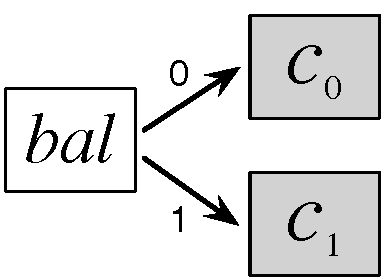
\includegraphics[width=2.1cm]{counter.pdf} 
\end{minipage}
&
\begin{minipage}[l]{4.9cm}
\centering
{\small{
\[
\begin{array}{rl}
\Num{1} & \esc{getAndInc()} : \esc{nat}~=~\esc{\{}  \\[2pt] 
\Num{2} & ~~~~ b \Asgn \esc{flip(}\bal\esc{)};\\[2pt]
\Num{3} & ~~~~ \res \Asgn \esc{fetchAndAdd2(}c_b\esc{)};\\[2pt]
\Num{4} & ~~~~ \kw{return}~\res~\esc{\}}
\end{array}
\]
}}
\end{minipage} 
%
\end{tabular}
%
\vspace{-10pt}  
\caption{Simple counting network}
\label{fig:counter-fig} 
%\vspace{-15pt}  
\end{figure}
}

Figure~\ref{fig:counter-fig} presents a schematic outline and a
pseudo-code implementation of a counting network with a single
balancer.
%
The implementation contains three pointers: the balancer $\bal$, which
stores either 0 or 1, thus directing threads to the shared pointers
$c_0$ or $c_1$, which count the even and odd values,
respectively. Threads increment by calling \code{getAndInc}, which
works as follows. It first atomically changes the bit value of the
balancer via a call to atomic operation \code{flip} (line 2). The
\code{flip} operation returns the \emph{previous} value $b$ of the
balancer as a result, thus determining which of the counters, $c_0$ or
$c_1$, should be incremented. The thread proceeds to atomically add 2
to the value of $c_b$ via \code{fetchAndAdd2} (line 3). The old value
of $c_b$ is returned as the result of the procedure.\footnote{In the
  counting network from Figure~\ref{fig:counter-fig}, the balancer
  itself might seem like a contention point. However, the \code{flip}
  operation is much less expensive than \code{CAS} as a
  synchronization mechanism. The performance can be further improved
  by constructing a \emph{diffracting tree} of several
  balancers~\cite[\S 12.6]{Herlihy-Shavit:08}, but we do not consider
  diffracting trees here.}

Assuming that $c_0$ and $c_1$ are initialized with $0$ and $1$, it is
easy to see that in a single-threaded program, the network will behave
as a conventional counter; that is, consecutive invocations of
\code{getAndInc} return consecutive nats.
%
However, in the concurrent setting, \code{getAndInc} may return
results out of order, as follows. 
%
% which historically led to the definition of quiescent
% consistency~\cite[\S 3.3]{Herlihy-Shavit:08} in order to specify the
% network's concurrent behavior.

\vspace{3pt}
\begin{example}
\label{ex:t1t2}
%
Consider two threads, $T_1$ and $T_2$ operating on the network
initialized with $\bal\,{\mapsto}\,0$, $c_b\,{\mapsto}\,b$. $T_1$
calls \code{getAndInc} and executes its line~2 to set $\bal$ to 1. It
gets suspended, so $T_2$ proceeds to execute lines~2 and~3, therefore
setting $\bal$ back to $0$ and returning $1$. While $T_1$ is still
suspended, $T_2$ calls \code{getAndInc} again, gets directed to $c_0$,
and returns 0, after it has just returned 1.
%
\end{example}
\vspace{3pt}

\noindent

This out-of-order behavior, however, is not random, and can be
precisely characterized as a function of the number of threads
operating on the
network~\cite{Afek-al:OPODIS10,Jagadeesan-Riely:ICALP14}. In the rest
of this section and in Section~\ref{sec:qclients}, we show how to
capture such bounds in the spec using auxiliary state of (subjective)
histories in a client-sensitive manner. As a form of road map, we list
the desired requirements for the spec of \code{getAndInc},
%
adapting the design goals of the criteria, such as QC, QQC and
QL~\cite{Aspnes-al:JACM94,Afek-al:OPODIS10,Jagadeesan-Riely:ICALP14},
which we will proceed to verify formally, following \textbf{\emph{Step
    1}} and \textbf{\emph{Step 2}} of our approach, and then employ in
client-side reasoning via \textbf{\emph{Step 3}}:
%
\vspace{2pt}
\begin{itemize}

\item \textbf{R1:} Two different calls to \code{getAndInc}
  should return distinct results (\emph{strong concurrent
    counter semantics}).

\item \textbf{R2:} The results of calls to \code{getAndInc},
  separated by a period of quiescence (\ie, absence of interference),
  should appear in their sequential order (\emph{quiescent
    consistency}).

\item \textbf{R3:} The results of two sequential calls $C_1$ and
  $C_2$, in a single thread should be out of order by no more than $2\
  N$, where $N$ is the number of interfering calls that overlap with
  $C_1$ and $C_2$ (\emph{quantitative quiescent consistency}).
%\an{Can we chose one of the two here: either qqc or ql?}

\end{itemize}

%\vspace{2pt}
%\lipsum[1]

\subsection{Step 1: counting network's histories and invariants}
\label{sec:counting-intuition}

To formalize the necessary invariants, we elaborate the counting
network with auxiliary state: \emph{tokens} (isomorphic to nats) and
novel \emph{interference-capturing histories}.

A \emph{token} provides a thread that owns it with the right to
increment an appropriate counter~\cite{Aspnes-al:JACM94}. In our
example, a thread that performs the \code{flip} in line 2 of
\code{getAndInc} will be awarded a token which it can then spend to
execute \code{fetchAndAdd2}.
%
Thus, any individual token represents a ``pending'' call to
\code{getAndInc}, and the set of unspent tokens serves as a bound on
the out-of-order behavior that the network exhibits. We introduce
auxiliary variables for the held tokens: $\tkns$ keeps the tokens
owned by the \emph{self} thread, with its \emph{even} and \emph{odd}
projections $\tkns^0$ and $\tkns^1$, such that $\tkns = \tkns^0
\hunion \tkns^1$, administering access to $c_0$ and $c_1$,
respectively. Similarly, $\tkno$, featuring the same projections,
keeps the tokens owned by the \emph{other} thread.  We abbreviate
$\tkn^i = \tkns^i \hunion \tkno^i$ for $i=0,1$.  
%
% \an{Is there a way to compute tokens out of some global
%   \emph{ordinary} history, so that we don't have to use an
%   \emph{interference-capturing} one? If not, we should stress the
%   point.}
%
% \is{I don't think there is, and I'm not sure if we have to elalorate
%   on this point.}

Figure~\ref{fig:chist} illustrates a network with three \emph{even}
tokens: $x^0, y^0, z^0 \in \tkn^0$, held by threads that will
increment $c_0$, and one \emph{odd} token $u^1 \in \tkn^1$, whose
owner will increment $c_1$.
%
%\an{Removed: We also point out here that token names (and their
%  uniqueness) will be of critical importance for the specifications we
%  give further. This point was never emphasized later on, so why
%  bother drawing attention to it.}

A \emph{history} of the counting network is an auxiliary finite map,
consisting of entries of the form $t \mapsto (\tknh, z)$.  Such an
entry records that the value $t$ has been written into an appropriate
counter ($c_0$ or $c_1$, depending on the parity of $t$), at the
moment when $\tkn^0$ and $\tkn^1$ held values of $\tknh$'s even/odd
projections $\tknh^0$ and $\tknh^1$, respectively. Moreover, in order
to write $t$ into a counter, the token $z$ was spent by the thread. We
will refer to $z$ as the \emph{spent} token. Notice that the entries
in the history contain tokens held by both \emph{self} and
\emph{other} threads. Thus, a history captures the behavior of a
thread subjectively, \ie, as a function of the interfering threads'
behavior.

Similarly to tokens, network histories are represented by the
auxiliary variables $\hists$, tracking counter updates (even and odd)
performed by the \emph{self} thread, and dually $\histo$ for the
\emph{other} thread. We abbreviate $\hist^i = \hists^i \hunion
\histo^i$ for $i = 0,1$.

Figure~\ref{fig:chist} illustrates a moment in network's history and
how it relates to the state of the counters. Only $0$ has been written
to $c_0$ so far (upon initialization), hence $\hist^0$ only contains
an entry for $t = 0$ (we ignore at the moment the \emph{contents} of
the history entries). On the other hand, $\hist^1$ has entries for $1$
and $3$, because after initialization, one thread has increased $c_1$.
%
The gray boxes indicate that $0$ and $3$ are the current values of
$c_0$ and $c_1$, and thus also the latest entries in $\hist^0$ and
$\hist^1$, respectively. In particular, these values will be returned
by the next invocations of \code{fetchAndAdd2}. The dashed boxes
correspond to the entries to be contributed by the currently running
threads holding tokens $x^0$, $y^0$, $z^0$, $u^1$.
%
% However, as thread scheduling is non-deterministic, we cannot predict
% which of the tokens will be spent to, say, write 2 into $c_0$ (it may
% be any even token).

{
\setlength{\belowcaptionskip}{-15pt} 
\begin{figure}
\centering
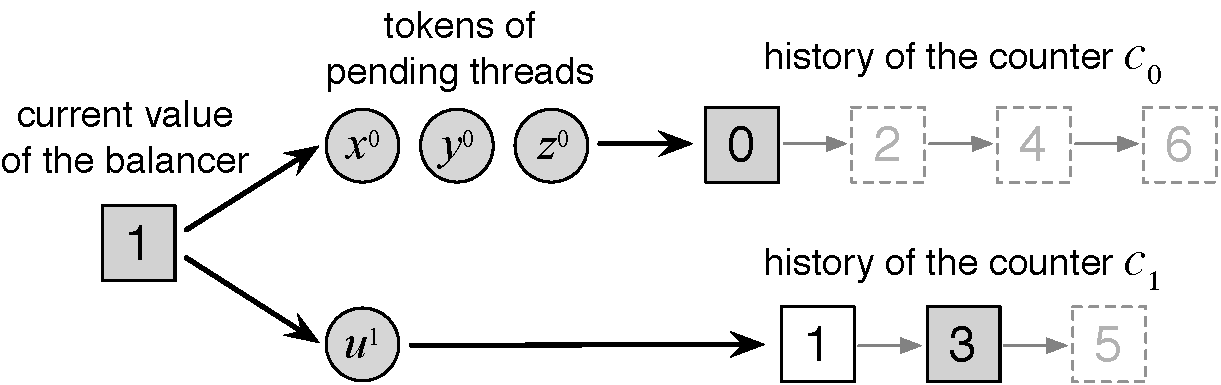
\includegraphics[width=8.2cm]{chist.pdf}      
\caption{Tokens and histories of the simple network}
\label{fig:chist}
\end{figure}
}




% We next list the invariants that describe the interdependence between
% the various components of the real and auxiliary state. 

In addition to $\tkn$ and $\hist$ which come in flavors private to
\emph{self} and \emph{other} threads, we require the following shared
variables: (1) $\heapj$ for the joint heap of the network, and (2)
$b_\joint$, $n^0_\joint$ and $n^1_\joint$ for the contents of $\bal$,
$c_o$ and $c_1$, respectively.

\paragraph{Invariants of the counting network}
\label{sec:count-netw-invar}

The main invariant of the network relates the number of tokens, the
size of histories and the value of the balancer:

\[
\tag{\normalsize{\arabic{tags}}}\refstepcounter{tags}\label{cn:si} 
%
|\hist^0| + |\tkn^0| =
|\hist^1| + |\tkn^1| + b_\joint
\]

The equation formalizes the intuition that out-of-order anomalies of
the counting network appear if one of the two counters is too far
ahead of the other one.
%
The invariant~(\ref{cn:si}) provides a bound on such a situation. One
counter can get ahead temporarily, but then there must be a number of
threads waiting to spend their tokens on the other counter. Thus, the
other counter will eventually catch up.

The approaches such as quiescent and quantitative quiescent
consistency describe this situation by referring to the number of
\emph{unmatched} call events in an event
history~\cite{Derrick-al:FM14,Jagadeesan-Riely:ICALP14}. In contrast,
we formalize this property via auxiliary state: the sets of tokens
$\tknh$ recorded in the entry for the number $t$ determine the
environment's capability to add new history entries, and thus ``run
ahead'' or ``catch up'' after $t$ has been returned.
%
% Such auxiliary state will let us directly specify the network's
% behavior in the moments of quiescence (\ie,~when $\tkno$ is empty),
% but also \emph{quantitatively} bound the out-of-orderness as a
% function of $\tkno$.
%
The other invariants of the counting network are as follows:
%\vspace{2pt}
\begin{enumerate}[label=(\roman*)]

% %
% \[
% \tag{\normalsize{\arabic{tags}}}\refstepcounter{tags}\label{eq:cn-states} 
% {\small
% \begin{array}{r@{\ }c@{\ }l} 
% {\!\!\!\!\!\!\!\!}W_{\ccon} & \!\eqdef & \exists \tkns~\tkno~ \hists~\histo~b~n_0~n_1\ldot 
% %  
% \qcl \spts (\tkns, \hists)\aand \qcl \opts (\tkno, \histo) 
%   \\[4pt] 
% &\aand & \qcl \jpts \bal \hpts b \hunion c_0 \hpts n_0 \hunion c_1 \hpts n_1   
%  \aand \hvalid~(\hists \hunion \histo)         \\[3pt] 
% &\aand & \SI~\tkn^0~\tkn^1~\hist^0~\hist^1~b ~~~~\aand
%          \CI~\hist^0~\hist^1~n_0~n_1 \\[3pt]  
% &\aand & \TI~\tkn^0~\tkn^1~(\hist^0 \hunion \hist^1)\aand \AI~\hist^0~\hist^1~\tkn^0~\tkn^1~n_0~n_1.
% \end{array}
% }
% \]
%

% where $\hist^i = (\hists \hunion \histo)^i$ and
% $\tkn^i = (\tkns \hunion \tkno)^i$ for $i \in \set{0,1}$.

\item\label{cn:state} $\heapj = \bal \mapsto b_\joint \hunion c_0 \mapsto n^0_\joint
  \hunion c_1 \mapsto n^1_\joint$.

\item\label{cn:hvalid} The histories contain disjoint time-stamps. % (\ie $\hists \hunion \histo$ is always defined);
 
% The state-space invariant $W_{\ccon}$ fixes the auxiliary self/other
% components to be pairs of tokens and histories $(\tkns, \hists)$ and
% $(\tkno, \histo)$, which are held/contributed by the thread and its
% environment, correspondingly. The invarian $\hvalid~(\hists \hunion
% \histo)$ ensures that at any moment 
% %
% The joint part of the state contains the pointers $\bal$, $c_0$ and
% $c_1$, and the relations between all these components are specified by
% the invariants $\SI$, $\CI$, $\TI$ and $\AI$.

\item\label{cn:ci} 
%
  The history $\hist^0$ (resp. $\hist^1$) contains \emph{all} even
  (resp. odd) values in $[0, n^0_\joint]$ (resp. $[1, n^1_\joint]$).
%
%    In other words, the network does not ``skip'' values. 
%
    This ensures that $n^0_\joint$ and $n^1_\joint$ are the last
    time-stamps in $\hist^0$ and $\hist^1$, respectively.

\item\label{cn:ti}  
%
  $\tkn^0$, $\tkn^1$ and $\Tomb~(\hists \hunion \histo)$ contain
  mutually disjoint tokens, where $\Tomb~(t \mapsto (\tknh, z) \hunion
  \hist') = \{z\} \hunion \Tomb~\hist'$, and $\Tomb~\emptyset =
  \emptyset$. In other words, a spent token never appears among the
  ``alive'' ones (\ie, in $\tkn^0 \hunion \tkn^1$).

%As a consequence, $\Tomb~(\hists \hunion \histo)$ is always defined.

\item\label{cn:ti1}
%
  $t \mapsto (\tknh, z) \subseteq \hists \hunion \histo
  \implies z \in \tknh$. \\[-7pt]

\item\label{cn:ai} 
%
For any $t$, $\tknh$, $z$: \\[-7pt]
% 
{\small
  \begin{itemize}
  \item   $t \hpts (\tknh, z) \subseteq \hist^0 \implies t + 2\ |\tknh
    \cap \tkn^0| < n^1_\joint + 2\ |\tknh \cap \tkn^1| + 2$, and \\[-7pt]
  \item
    $t \hpts (\tknh, z) \subseteq \hist^1 \implies t + 2\ |\tknh \cap 
    \tkn^1| < n^0_\joint + 2\ |\tknh \cap \tkn^0|
    + 2$.
  \end{itemize}
}
%
\end{enumerate}
\vspace{5pt}
 
\noindent
The invariant~\ref{cn:ai} provides quantitative information about the
network history by relating the actual ($n^0_\joint$, $n^1_\joint$)
and the past ($t$) counter values, via the current amount of
interference ($\tkn$) and the snapshot interference ($\tknh$).
%
To explain~\ref{cn:ai}, we resort to the intuition provided by the
following equality, which, however, being \emph{not quite valid},
cannot be used as an invariant, as we shall see. Focusing on the
first clause in~\ref{cn:ai}, if
$t \mapsto (\tknh, z) \subseteq \hist^0$, then,
intuitively:
%
{\small{
\[
t + 2\ |\tknh^0 \setminus \tkn^0 | + 2\ |\tknh \cap \tkn^0| =
n^1_\joint + 2\ |\tknh \cap \tkn^1| + (2 b_\joint - 1)
\]}}
%
\noindent
The equality says the following. When $t$ is snapshot from $c_0$ and
placed into the history $\hist^0$, the set of outstanding even tokens
was $\tknh^0$. By the present time, $c_0$ has been increased
$|\tknh^0 \setminus \tkn^0|$ times, each time by $2$, thus
$n^0_\joint = t + 2\ |\tknh^0 \setminus \tkn^0|$. What is left to add
to $c_0$ to reach the \emph{period of quiescence}, when no threads
interfere with us, is $2\ |\tknh \cap \tkn^0|$. Similar reasoning
applies to $c_1$. It is easy to see at the period of quiescence, $c_0$
and $c_1$ differ by $2 b_\joint - 1$; that is, the counter pointed to
by $\bal$ is behind by $1$. However, the equality is invalid, as
$b_\joint$ can be read off only in the present, whereas the
``intuitive'' reasoning behind the equality requires a value of
$b_\joint$ from a quiescent period \emph{in the future}. Hence, in
order to get a valid property, we bound $2 b_\joint - 1$ by 2. For
simplicity, we even further weaken the bounds by dropping
$|\tknh^0 \setminus \tkn^0|$ to obtain~\ref{cn:ai}; as it will turn
out, even such a simpler bound will suffice for proving
\textbf{R1}--\textbf{R3}.

% in Section~\ref{sec:qc-client}.

%As already aparent from our explanation, the invariant gives us a way
%to formally model when the network is in the period of quiescence, as
%required in \textbf{R2}, which we verify in
%Section~\ref{sec:qc-client}.
%%

% \gad{I did not find the equation above ``intuitive'' at all. I think
%   it might be better to give the first part of the explanation and
%   introduce the equality. Then, say why it doesn't hold and how to fix
%   it to get a valid invariant. I think that would be easier to
%   understand.}
%
% wontfix
%
% \gad{Also, why the quotation marks around equation? Valid or not, it
%   is still an equality.}
%
% won't fix

\paragraph{Allowed changes in the counting network}
\label{sec:count-netw-prot}


The state of the counting network (auxiliary and real) can be changed
in two possible ways by concurrent threads. These changes formalize
the way the atomic operations \code{flip} and \code{fetchAndAdd2} from
Figure~\ref{fig:counter-fig}~(b) work with auxiliary state.
%
\emph{Flipping} alters the bit value $b_\joint$ of $\bal$ to the
complementary one, $1 - b_\joint$.
%
It also generates a token $z$ (of parity $b_\joint$) and stores it
into $\tkns$. The token is fresh, \ie, distinct from all alive and
spent tokens in $\tkns \hunion \tkno \hunion{\Tomb~(\hists
  \hunion \histo)}$.
%
\emph{Incrementation} spends a token $z$ from $\tkns$, and depending
on its $i$, it atomically increases the value $n^i_\joint$ of $c_i$ by
two, while simultaneously removing $z$ from $\tkns$ (thus, the
precondition is that $z \in \tkns$). It also adds the entry
$(n^i_\joint + 2) \hpts (\tkn^0 \hunion \tkn^1, z^i)$ to $\hists$,
thus snapshoting the values of $\tkn^0$ and $\tkn^1$.
%
It is easy to check that both these allowed changes preserve the
state-space invariants~(\ref{cn:si}), \ref{cn:state}--\ref{cn:ai}, and
that their effect on real state (with auxiliary state erased) are
those of \code{flip} and \code{fetchAndAdd2}.

\subsection{Step 2: a Hoare spec for \texttt{getAndInc}}
\label{sec:spec-gaa}

We now provide a Hoare-style spec for \code{getAndInc}, verified in
our proof scripts. We use the logical variable $\ikn$ and its variants
to range over token sets, and $\gist$ to range over histories.

\[
%
\tag{\normalsize \arabic{tags}}\refstepcounter{tags}\label{eq:qc-spec}
{\small
\!\!\!\!\!\!\!\! 
\begin{array}{c}
  \spec{\!\!
  \begin{array}{c}
    \tkns = \emptyset,
    \hists = \gists,
    \gisto \subseteq \histo,\\[2pt]
    \ikno \subseteq \tkno \hunion (\Tomb~\histo \setminus
    \Tomb~\gisto),
    \Ic{\gisto}{\ikno}
  \end{array}
  \!\!}
  \\\\[-6pt]
  \texttt{getAndInc()}
  % 
  \\[3pt]
  \spec{\!\!\!
  \begin{array}{c}
    \exists \iknh~z \ldot \tkns = \emptyset, 
    \hists = \gists \hunion (\res + 2) \hpts (\iknh, z), 
    \\[2pt]
    \gisto \subseteq \histo, \ikno \subseteq \tkno \hunion (\Tomb~\histo \setminus \Tomb~\gisto), 
    \\[2pt]
    \last~(\gists \hunion \gisto) < 
    \res + 2 + 2~|\iknh \cap \ikno|, 
    \\[2pt]
    \happrox~(\gists \hunion \gisto)~\res~\iknh~z,
     \Ic{\gisto}{\ikno}
  \end{array} 
  \!\!\!} %@\ccon
%
\end{array}
}
\]

The precondition starts with an empty token set ($\tkns = \emptyset$),
and hence by framing, any set of tokens. The initial self-history
$\hists$ is set to an arbitrary $\gists$.\footnote{Alternatively, we
  could have also taken $\hists = \emptyset$, but the clients will
  require generalizing to $\hists = \gists$ by the FCSL's frame
  rule~\cite{Sergey-al:ESOP15}. To save space and simplify the
  discussion, we immediately frame \wrt the auxiliary $\hists$. Our
  examples do not require such client-side framing \wrt~$\tkns$.} The
precondition records the \emph{other} components of the initial state
as follows. First, $\gisto$ names (a subset of) $\histo$, to make it
stable under interference, as in Section~\ref{sec:overview}. Next, we
use $\ikno$ to name the (subset of) initially live tokens
$\tkno$. However, as $\tkno$ may shrink due to other threads spending
tokens, simply writing $\ikno \subseteq \tkno$ is unstable. Instead,
we write $\ikno \subseteq \tkno \hunion (\Tomb~\histo \setminus
\Tomb~\gisto)$ to account for the tokens spent by other threads as
well. The set $\tkno \hunion (\Tomb~\histo \setminus \Tomb~\gisto)$
only grows under interference, as new live tokens are generated, or
old live tokens are spent, making the inclusion of $\ikno$ stable.
%
Indeed, one cannot take \emph{any} arbitrary $\gisto$ and $\ikno$ to
name the \emph{other} components of the initial state. Therefore, we
constrain these two variables by the invariant $\ic$, that relates
them to the \emph{self-}components of the actual state and to each
other according to the
invariants~\ref{cn:hvalid}--\ref{cn:ai}.\footnote{That is, $\gisto$
  and $\ikno$ take the role of $\histo$ and $\tkno$ in
  invariants~\ref{cn:hvalid}--\ref{cn:ai}, with
  $n^i_\joint = \last~(\hists \hunion \gisto)^i$. The formal
  definition of $\ic$ is in our proof scripts.} This is natural,
since, as we will see in Section~\ref{sec:qclients}, all clients
instantiate $\gisto$ and $\ikno$ with the \emph{other}-components of
the actual pre-state, respecting~\ref{cn:hvalid}--\ref{cn:ai}.

% \gad{$ \ikno \subseteq \tkno \hunion (\Tomb~\histo \setminus
%   \Tomb~\gisto)$ breaks awkwardly across lines.}
% wontfix
%
% \gad{I don't get the parentheses around ``a subset of''. It makes it
%   harder to read the phrases, and after all the full subset is still a
%   subset.}
%
% fixed
%
% \gad{I did not get what $\Ic{\gisto}{\ikno}$ is, even after browsing
%   the spec in the code. Is it too long to define it inline? Does it
%   matter altogether?}
%
%   Yes, it does matter. And, yes, it's too long to define it in
%   prose, as it's boring and comes from the fact that SL-ish notation
%   is not a good fit for binary state-constrining postconditions.
%

The postcondition asserts that the final token set $\tkns$ is also
empty (\ie, the token that \code{getAndInc} generates by \code{flip},
is spent by the end). The history $\hists$ is increased by an entry
$(\res + 2) \hpts (\iknh, z)$, corresponding to writing the value of
the result (plus two) into one of the network's counters, snapshoting
the tokens of that moment into $\iknh$, and spending the token $z$ on
the write. $\gisto$ is a subset of the new value of $\histo$, and
$\ikno$ is a subset of the new value of $\tkno \hunion (\Tomb~\histo
\setminus \Tomb~\gisto)$, by the already discussed stability.

The next inequality describes where the entry for $\res + 2$ is placed
\wrt~the pre-state history $\gist = \gists \hunion \gisto$. $\gist$
may have gaps arising due to out-of-order behavior of the network, and
$\res + 2$ may fill one such gap. However, there is a bound on how far
$\res$ (and hence $\res+2$) may be from the tail of $\gist$. We
express it as a function of $\ikno$ and $\iknh$, derived from the
bounds in~\ref{cn:ai}, taking $\res + 2$ for $t$ and
over-approximating the instant value $n_{\joint}^i$ of the
incremented counter via $\last~(\gists \hunion \gisto)$. The
inequality weakens the invariant~\ref{cn:ai}, making it hold for even
and odd entries by moving $2~|\iknh \cap \ikno^i|$ (for $i = 0,1$) to
the right side of $<$ and joining them, since $\ikno^0 \cap \ikno^1 =
\emptyset$.

% To explain it, let us assume that $\res$ is written into $c_1$ and the
% last entry of $\hist$ (let us call it $t$) was written into
% $c_0$. Then, we have a similar ``equation'' as in the explanation
% in~\ref{cn:ai}:
% \[
% t + 2\ |\ikno^0 \setminus \iknh^0| + 2\ |\iknh^0 \cap \ikno^0| = \res
% + |\iknh^1 \cap \ikno^1| + (2 b_\joint -1)
% \]
% To advance $c_0$ to the moment when $\iknh^0$ and $\iknh^1$ were
% recorded, we need to increase $t$ by $2\ |\ikno^0 \setminus
% \iknh^0|$. After that, to advance both $c_0$ and $c_1$ to a quiescent
% period, we have to spend the tokens in $|\iknh^0 \cap \ikno^0|$ (for
% $c_0$) and $|\iknh^1 \cap \ikno^1|$ (for $c_1$). In the quiescent
% period, $c_0$ and $c_1$ differ by $2 b_\joint - 1$. Moving $|\iknh^0
% \cap \ikno^0|$ to the other side of the equation (while not changing
% the sign), omitting $|\ikno^0 \setminus \iknh^0|$, and bounding the
% value of $2 b_\joint - 1$ from above by $2$, we get:
% \[
% t < \res + 2\ |\iknh^0 \cap \ikno^0| + 2 \ |\iknh^1 \cap \ikno^1| + 2
% \]
% which we use in~(\ref{eq:qc-spec}). Being symmetric in $\ikn^0$ and
% $\ikn^1$, the inequality has the pleasant property that it also holds
% in the other three cases: when $\res$ is written into $c_0$ and $t$
% into $c_1$, and when both $\res$ and $t$ are written into the same
% counter, $c_0$ or $c_1$.

% The predicate $\strapprox$, stated next, summarizes several properties
% of the result and the newly introduced history entry, which will be
% crucial for reasoning about clients in Section~\ref{sec:qclients}:
% %
% \[
% \tag{\normalsize \arabic{tags}}\refstepcounter{tags}\label{eq:strapprox}
% %
% \!\!\!\!
% {\small{
% \begin{array}{l}
% \strapprox~\gists~\gisto~\ikno~m_0~m_1~\res~\iknh^0~\iknh^1~z
% ~\eqdef
% \\[2pt]
% ~~~~~~~~~~~~~~~~~~ \sapprox~\ikno~m_0~m_1~\res~\iknh^0~\iknh^1, \\[2pt]
% ~~~~~~~~~~~~~~~~~~ \happrox~(\gists \hunion \gisto)~\res~\iknh^0~\iknh^1~z,\\[2pt]
% ~~~~~~~~~~~~~~~~~~ \tapprox~(\gists \hunion \gisto)~\iknh^0~\iknh^1~z
% \end{array}
% }}
% \]
% %
% \[
% %
% \tag{\normalsize \arabic{tags}}\refstepcounter{tags}\label{eq:sapprox}
% %
% {\small{
% \begin{array}{l}
% \sapprox~\ikn~m_0~m_1~\res~\iknh^0~\iknh^1 ~\eqdef \\[2pt]
% %
% ~~~~  m_0 < \res + 2 + 2 \times (|\iknh^0 \cap \ikn^0| + |\iknh^1 \cap
%   \ikn^1|), \\[2pt]
% ~~~~ m_1 < \res + 2 + 2 \times (|\iknh^0 \cap \ikn^0| + |\iknh^1 \cap
%   \ikn^1|)
% \end{array}
% \hfill
% }}
% \]
% 

%\noindent
Finally, the predicate $\happrox$ provides more bounds that we will
need in the proofs of the client code's properties.
%
\[ 
%
\tag{\normalsize \arabic{tags}}\refstepcounter{tags}\label{eq:happrox}
%
\!\!\!\!\!
{\small{
\begin{array}{l}
\!\!\!\!
\happrox~\gist~\res~\iknh~z \eqdef \hbox{}
\iknh \subseteq \tkno \hunion (\Tomb~\histo) \hunion
  \set{z},\\[2pt]
~~ \forall t~\ikn \ldot t \hpts (\ikn, -) \subseteq \gist \Rightarrow
  z \notin \ikn,~  t < \res + 2 + 2 \ (|\iknh \cap \ikn|)
\end{array}
}}
\]
%
When instantiated with $\gist = \gists \hunion \gisto$, $\happrox$
says the following. The token set $\iknh$ snapshot when $\res+2$ was
committed to history, is a subset of all the tokens in post-state,
including the live ones ($\tkno$), and spent ones ($\Tomb~\histo
\hunion \{z\}$).
%
Moreover, if $t$ is an entry in $\gist$, with contents $(\ikn, -)$,
then: (1) $z \notin \ikn$, because $z$ is a token generated when
\code{getAndInc} executed \code{flip}. Hence, $z$ is fresh \wrt~any
token-set from the pre-state history $\gist$; and (2) $t$ and $\ikn$
satisfy the same bounds \wrt~$\res+2$, as those described for the last
history entry and~$\ikno$.


%\noindent

%
% \begin{comment}
% \paragraph{Why the spec~\eqref{eq:qc-spec} is stable?}
% \label{sec:why-spec-eqrefeq:qc}

% The stability of the spec we ascribed to \code{getAndInc} follows from
% the following observations. First, all clauses in the pre- and
% postconditions that contsrain only \emph{self}-components of the state
% (\eg, $s.\hists = \gists$ or $\tkns = \emptyset$) are stable, since
% they cannot be affected by interference (which might change only
% \emph{other} and \emph{joint} components), as ensured by FCSL's
% meta-theory.
% %
% Second, the stability of all other clauses that also mention the
% \emph{other} component, follows from their \emph{monotonicity} with
% respect to interference. In particular, the union
% $\tkno \hunion \Tomb~\histo$, appearing also in the definition of
% $\happrox$, can only grow, while the union
% $\ikno \hunion \Tomb~\gisto$ is fixed.
% %
% Finally, the rest of the clauses mentions only values that are not
% components of the state being constrained (\eg, $\ikno$, $\gisto$,
% \etc) and, hence, are also unaffected by interference.
% %
% All these stability arguments are carried out as formal proofs in our
% Coq development, accompanying the paper.
% \end{comment}

\paragraph{How will the spec~\eqref{eq:qc-spec} be used?}

The clause $\hists\,{=}\,\gists \hunion (\res+2)\,{\mapsto}\,-$ of
\eqref{eq:qc-spec}, in conjunction with the invariant~\ref{cn:hvalid},
ensures that any two calls to \code{getAndInc}, sequential or
concurrent, yield different history entries, and hence different
results. This establishes~\textbf{R1}, which we will not discuss
further.

The inequality on $\last~(\gists \hunion \gisto)$ will provide
for~\textbf{R2} in client reasoning. To see how, consider the
particular case when $\ikno$ is empty, \ie, the pre-state is
quiescent. In that case, the intersection with $\iknh$ is empty, and
we can infer that $\res + 2$, is larger than either counter's value in
the pre-state. As we shall see in Section~\ref{sec:qclients}, this
captures the essence of QC.

Finally, the predicate $\happrox$~\eqref{eq:happrox} establishes a
bound for the ``out-of-order'' discrepancy between the result $\res$
and any value $t$ committed to the history \emph{in the past}, via
$2~|\iknh \cap \ikn|$. We will further bound this value using the size
of $\iknh$, and the inclusion $\iknh \subseteq \tkno \hunion
\Tomb~\histo$ from~\eqref{eq:happrox}. These bounds will ultimately
enable us to derive the requirement~\textbf{R3}.

% \gad{ The $\hists \ldots$ clause line-breaks bad.}

% \subsubsection{Specifications of {\code{flip}} and
%   {\code{fetchAndAdd2}}}
% \label{sec:qacts}

% The formal verification of the spec~\eqref{eq:qc-spec} follows by
% sequential composition of its operations, \code{flip} and
% \code{fetchAndAdd2}, to which we ascribe the following specs.
% %
% Both specs are obtained by relaxing the definitions of the transitions
% from Section~\ref{sec:count-netw-prot}, \wrt~stability.
% %
% %
% \[
% %
% %\tag{\normalsize \arabic{tags}}\refstepcounter{tags}\label{eq:flip-spec}
% {\small
% %\!\!\!\!\!\!\!\! 
% \begin{array}{c}
%   \spec{\!\!
%   \begin{array}{c}
%     \tkns = \emptyset,
%     \hists = \gists,
%     \gisto \subseteq \histo,\\[2pt]
%     \ikno  \subseteq \tkno \hunion (\Tomb~\histo \setminus
%     \Tomb~\gisto), 
%      \Ic{\gisto}{\ikno}
%   \end{array}
%   \!\!}
%   \\\\[-6pt]
%   \texttt{flip(}\bal\texttt{)}
%   %  
%   \\[3pt]
%   \spec{\!\!
%   \begin{array}{c}
%     \exists b~z^b \ldot \res = (b, z^b)\aand
%     \tkns = \set{z^b}\aand \hists = \gists \aand
%      \Ic{\gisto}{\ikno},
%    \\[2pt]
%     \gisto \subseteq \histo, \ikno \subseteq \tkno \hunion (\Tomb~\histo \setminus \Tomb~\gisto),\\[2pt]    
%     \forall t~\ikn^0~\ikn^1 \ldot
%     t \hpts (\ikn^0, \ikn^1, -) \subseteq (\gists \hunion \gisto) \Rightarrow z^b \notin \ikn^0 \hunion \ikn^1,
%     \\[2pt]     
%     \bapprox~(\last~(\gists \hunion \gisto)^0)~(\last~(\gists \hunion \gisto)^1)~\ikno 
%   \end{array}
%   \!\!}@\ccon
% %
% \end{array}
% }
% \]

% \noindent
% The precondition of \code{flip}'s matches the one of
% \code{getAndInc}. The postcondition contains a clause with a new
% predicate $\bapprox$, relating the last entries $m_0$ and $m_1$ of
% either parity of the initial history $\gist = \gists \hunion \gisto$,
% to the current values $n_\joint^0$ and $n_\joint^1$ of $c_0$ and
% $c_1$.
% %
% \[
% %
% \!\!\!\!
% {\small{
% \begin{array}{l}
% \bapprox~m_0~m_1~\ikno \eqdef \\[2pt]
% %
%   \begin{array}{l}
%    m_0 \le n_\joint^0\aand
%     m_1 + 2 \times |\ikno^1 \cap \tkn^1| < n_\joint^0 + 2 \times
%   |\ikn^0 \cap  \tkn^0| + 2, \\[2pt]
%    m_1 \le n_\joint^1\aand m_0 + 2 \times |\ikno^0 \cap \tkn^0| < n_\joint^1 + 2 \times
%   |\ikn^1 \cap  \tkn^1| + 2 
%   \end{array}
% \end{array}
% \hfill
% }}
% \]
% %
% The predicate says that the contents of $c_0$ and $c_1$ increases,
% hence $m_0$ and $m_1$ are smaller or equal to the current values
% $n_\joint^0$ and $n_\joint^1$, respectively. Moreover, when comparing
% values of different parities (\ie, $m_1$ with $n_\joint^0$ and $m_0$
% with $n_\joint^1$), we require bounds similar to the ones already
% discussed in~\ref{cn:ai} and~\eqref{eq:qc-spec}, and expressed in
% terms of token set $\ikno$ and $\tkn = \tkns \hunion \tkno$, that
% capture the interference in the pre-state and post-state,
% respectively. The predicate is internal to \esc{getAndInc}, and is not
% used by, or even visible to, the clients.

% The precondition of \code{fetchAndAdd2} is the same as \code{flip}'s
% postcondition, and \code{fetchAndAdd2}'s post is the one of
% \code{getAndInc}, so verifying the sequential composition is
% straightforward.
% %
% % We note that the $\bapprox$ property is essential for deriving the
% % inequalities from the postcondition~\eqref{eq:qc-spec}.
% %
% \[
% %
% %\tag{\normalsize \arabic{tags}}\refstepcounter{tags}\label{eq:add-spec}
% {\small
% %\!\!\!\!\!\!\!\!\!\! 
% \begin{array}{c}
%   \spec{\!\!
%   \begin{array}{c}
%    \tkns = \set{z^b}\aand \hists = \gists, 
%      \Ic{\gisto}{\ikno} \aand   \\[2pt]
%     \gisto \subseteq \histo, \ikno  \subseteq \tkno \hunion (\Tomb~\histo \setminus \Tomb~\gisto),\\[2pt]
%     \forall t~\ikn^0~\ikn^1 \ldot
%     t \hpts (\ikn^0, \ikn^1, -) \subseteq (\gists \hunion \gisto) \Rightarrow z^b \notin \ikn^0 \hunion \ikn^1,
%     \\[2pt]    
%     \bapprox~(\last~(\gists \hunion \gisto)^0)~(\last~(\gists \hunion \gisto)^1)~\ikno 
%   \end{array}
%   \!\!}
%   \\\\[-5pt]
%   \texttt{fetchAndAdd2($c_b, \specK{z^b}$)} 
%   % 
%   \\[3pt]
%   {\normalsize{ 
%   \specK{\{}~ {\small\texttt{getAndInc}}\specK{\text{'s post~\eqref{eq:qc-spec},
%   instantiated with}~\gists, \ikno, \gisto\}}@\ccon
%   }}
% %
% \end{array}
% }
% \]

% \noindent
% We note one peculiarity, however. In order to provide a provable spec
% for \code{fetchAndAdd2}, we had to augment its signature with a
% \emph{logical} parameter $\specK{z^b}$, representing the token,
% obtained by executing \code{flip}, to be spent in incrementation of
% $c_b$. While in most Hoare-style specs, logical variables scope over
% the precondition and the postcondition, but do not appear in the code,
% here we had to pass $z^b$ as a function argument.
% %
% This logical parameter serves purely for verification purposes, and
% does not affect the result of the execution. Hence, in principle, it
% can be safely erased, though our current formalization of FCSL in Coq
% does not support such erasure.




\section{Verifying Counting Network's Clients}
\label{sec:qclients}

% We next demonstrate how the spec~\eqref{eq:qc-spec} can be used in
% clients, to establish properties \textbf{R2} and \textbf{R3}. These
% properties have been addressed in the previous work using dedicated
% consistency criteria of quiescent
% consistency~\cite{Aspnes-al:JACM94,Derrick-al:FM14} and quantitative
% quiescent consistency and
% quasi-linearizability~\cite{Afek-al:OPODIS10,Jagadeesan-Riely:ICALP14},
% but here we derive them compositionally, \ie, out of the spec of
% \code{getAndInc}. This will demonstrate the usefulness of Hoare logic
% in deriving properties related to the various flavors of quiescent
% consistency.

Following \textbf{\emph{Step 3}} of our verification method, we now
illustrate requirements \textbf{R2} and \textbf{R3} from the previous
section via two different clients which execute two sequential calls
to \code{getAndInc}. Both clients are higher-order, \ie, they are
parametrized by subprograms, which can be ``plugged in''.
%
The first client will exhibit a quiescence between the two calls, and
we will prove that the call results appear in order, as required by
\textbf{R2}. The second client will experience interference of a
program with a $N$ concurrent calls to \code{getAndInc}, and we will
derive a bound on the results in terms of $N$, as required by
\textbf{R3}.

Both our examples will rely on the general mechanism of hiding,
presented in Section~\ref{sec:background}, as a way to logically restrict the
interference on a concurrent object, in this case, a counting network,
in a lexically-scoped way.
%
To ``initialize'' the counting network data structure, we provide the
starting values for the shared heap ($h_0$) and for the history
($\gist_0$), assuming that the initial set of tokens is empty:
%
% Specifically, we will use the following derived rule:
% %
% {\small{
% \[
% \begin{array}{c}
% \spec{P}~e~\spec{Q} @ \ccon\\[2pt]
% \hline\\[-7pt]
% \!\!\!
% \specK{\{\heaps = \Phi_1(\heapj), \Phi_1(P)\}} \hide_{\Phi_1}~e \specK{\{\exists \Phi_2\ldot \heaps = \Phi_2(\heapj), \Phi_2(Q)\}} @ \cal P
% \end{array}
% \]
% }}
%
\[
\tag{\normalsize \arabic{tags}}\refstepcounter{tags}\label{eq:hide2}
{\small{
\begin{array}{r@{\ }c@{\ }l}
% \text{\normalsize{where}} &
% \Phi_1 & \eqdef & [\emptyset/\tkns, \gist_0/\hists, \heap_0/\heapj,
% \emptyset/\tkno, \histo/\hists] 
% \\[2pt]
\heap_0 & \eqdef & \bal \hpts 0 \hunion c_0 \hpts 0 \hunion c_1 \hpts 1     
\\[2pt]
\gist_0 & \eqdef & \set{0 \hpts (\set{0}, 0), 1 \hpts (\set{1}, 1)}
\end{array}
}}
\]
%
That is, $\gist_0$ provides the ``default'' history for the initial
values 0 and 1 of $c_0$ and $c_1$, with the corresponding tokens
represented by numbers 0 and 1.  As always with hiding, the
postcondition of the hidden program will imply that $\tkno$ and
$\histo$ are both empty, as there is no interference at the end.

% \gad{I think that here, again, the quotation marks around ``plugged in'',
%   ``initialize'', and ``default'' are unnecessary.}

\subsection{Exercising quiescent consistency}
\label{sec:qc-client}

\begin{figure}
\centering
\[
{\small{
\!\!\!\!\!\!\!\!
\begin{array}{c}
  \spec{\!\!
  \begin{array}{c}
    \tkns = \emptyset,
    \hists = \gists,
    \gisto \subseteq \histo, \Ic{\gisto}{\ikno}, \\[2pt]
    \ikno \subseteq \tkno \hunion (\Tomb~\histo \setminus \Tomb~\gisto)
  \end{array}
  \!\!}
\\\\[-5pt]
  \begin{tabular}{c || c}
   $\esc{getAndInc()}$ & ${\small{e_i}}$ 
\end{tabular}
\\\\[-5pt]
~~~~\spec{\!\!
\begin{array}{c}
  \exists \iknh~\gist_i \ldot  
  \tkns = \emptyset\aand \hists = \gbm{\gists \hunion \gist_i \hunion (\res.1 + 2) \hpts (\iknh, -)},\\[1pt]
  \gisto \subseteq \histo\aand \ikno \subseteq \tkno \hunion
  (\Tomb~\histo \setminus \Tomb~\gisto), \Ic{\gisto}{\ikno},\\[1pt]
  \last~(\gists \hunion \gisto)  < \gbm{\res.1} + 2 +
  2~|\iknh \cap \ikno|
%
\end{array}
\!\!} %@\ccon
%
\end{array}
}}  
\]
%
\caption{Parallel composition of \code{getAndInc} and~$e_i$ in~\eqref{eq:eqc}.}
  \label{fig:example1} 
\end{figure}
%



Our first client is the following program~$\eqc$:
%
\[
\tag{\normalsize \arabic{tags}}\refstepcounter{tags}\label{eq:eqc}
{\small{
\begin{array}{ll} 
\Num{1} & (\res_1, -) \Asgn (\esc{getAndInc()} ~||~ e_1) \esc{;} \\[1pt]
\Num{2} & (\res_2, -) \Asgn (\esc{getAndInc()} ~||~ e_2) \esc{;} \\[1pt]
\Num{3} &  \kw{return}~(\res_1, \res_2) 
\end{array}
}}
\]
%
Each of the calls to \esc{getAndInc} interferes with either $e_1$ or
$e_2$, but in the absence of \emph{external} interference, the
quiescent state is reached between the lines 1 and 2. Hence, after
executing $\hide~\eqc$, it should be $\res_1 < \res_2$, following
\textbf{R2}.

The programs $e_1$ and $e_2$ can invoke \code{getAndInc} and modify
the counters concurrently with the two calls of $\eqc$, which we
capture by giving both the following generic spec:
%
\[
%
\tag{\normalsize \arabic{tags}}\refstepcounter{tags}\label{eq:eispec}
{\small
\!\!\!\!\!\!\!\! 
\begin{array}{c}
  \spec{~
  \hists = \emptyset\aand
  \tkns = \emptyset\aand
   \ikn \subseteq \tkno \hunion \Tomb~\histo
  ~}
  \\[1pt]
  e_i
  % 
  \\[1pt]
  \spec{\!\!\!
  \begin{array}{c}
    \exists \gist_i \ldot \hists = \gist_i\aand 
    \tkns = \emptyset\aand 
    \ikn \subseteq \tkno \hunion \Tomb~\histo
  \end{array} 
  \!\!\!} %@\ccon
%
\end{array}
}
\]
%
The postcondition allows for a number of increments via calls to
\esc{getAndInc}, which is reflected in the addition $\gist_i$ to
$\hists$. However, all such calls are required to be \emph{finished}
by the end of $e_i$ ($\tkns = \emptyset$). As customary by now, we use
the logical variable $\ikn$ to name the initial set of \emph{other}
tokens.

Figure~\ref{fig:example1} provides a spec for each of the parallel
compositions in the program~\eqref{eq:eqc}, proved via the
corresponding FCSL inference rule for parallel
composition~\eqref{eq:parrule}.
%
The spec is very similar to~\eqref{eq:qc-spec} with the differences
highlighted via gray boxes: (a) the self-history $\hists$ is increased
by $e_i$'s contribution $\gist_i$ in addition to the entry, introduced
by \code{getAndInc}, (b) the result of the parallel composition is a
pair, but we only constrain its first component $\res.1$, resulting
from the left subprogram. We also drop the last conjunct with
$\happrox$ from~\eqref{eq:qc-spec}, which we won't require for this
example.

%



Next, we use the spec from Figure~\ref{fig:example1} to specify and
verify the program $\eqc$, so far \emph{assuming} external
interference.
%
\[
\!\!\!
{\small{
\begin{array}{c}
\!\!\!\!\!
\spec{\!\!
  \begin{array}{c}
    % \tkns = \emptyset,
    % \gisto \subseteq \histo, \ikno \subseteq \tkno \hunion (\Tomb~\histo \setminus \Tomb~\gisto)\\[2pt]
    % \hists = \gist_0,
    \mbox{Fig.~\ref{fig:example1}'s precondition with $\gists := \gist_0$, $\gisto :=
      \histo$, and $\ikno := \tkno$}
  \end{array}
  \!\!}
  ~\comm{P}
  \\\\[-6pt]
  (\res_1, -) \Asgn (\esc{getAndInc()} ~||~ e_1) \esc{;}
  \\[3pt]
\!\!\!\!{{
\spec{\!\!\!\!
\begin{array}{c}
 \exists \gist_1\ldot \tkns = \emptyset\aand \hists = \gists',~\ldots
% \ikno \subseteq \tkno \hunion (\Tomb~\histo \setminus \Tomb~\gisto),
\\[2pt]
\mbox{where 
 $\gbm{\gists' = \gist_0 \hunion
\gist_1 \hunion (\res_1 + 2)\mapsto -}$, $\gisto := \histo$ and $\ikno :=
\tkno$} 
% \\[2pt]
% \mbox{hence $\Ic{\gisto}{\ikno}$}
  \end{array}
\!\!\!\!}
}}
%
\\\\[-5pt]
(\res_2, -) \Asgn (\esc{getAndInc()} ~||~ e_2) \esc{;}      
\\[3pt]
\spec{\!\!\!\!
\begin{array}{c}
\exists \gist_1~\gist_2~\iknh \ldot     
%
\tkns = \emptyset \aand 
%%\hists = \gists' \hunion \gist_2 \hunion (\res_2 + 2)\mapsto (\iknh, -)\aand\hbox{}\\[2pt] 
\gbm{\ikno \subseteq \tkno \hunion (\Tomb~\histo \setminus \Tomb~\gisto)},\\[1pt]
\gbm{\last~(\gists' \hunion \gisto) < \res_2 + 2 + 2~|\iknh \cap \ikno|},~\ldots 
\end{array}
\!\!\!\!\!}~\comm{Q}
\\\\[-7pt]
~~~~~~~~~~~\kw{return}~(\res_1, \res_2); ~\comm{=: \res} 
\\[2pt]
\spec{~Q(\res.1/\res_1, \res.2/\res_2)~} %@\ccon
\end{array}
}} 
\]
%
We start by instantiating the logical variables $\gists$, $\gisto$ and
$\ikno$ from Figure~\ref{fig:example1} with $\gist_0$, \emph{current}
$\histo$ and $\tkno$, respectively, naming the obtained precondition
$P$.
%
In the following assertion we focus on the clauses constraining
$\tkns$ and $\hists$. To verify the second call, we instantiate
$\gists$, $\gisto$ and $\ikno$ from Figure~\ref{fig:example1} with
$\gists' = \gist_0 \hunion \gist_1 \hunion (\res_1 + 2)\mapsto -$,
\emph{current} $\histo$ and $\tkno$, correspondingly, obtaining the
postcondition, which we name~$Q$.

The inequality in the postcondition $Q$ gives the boundary on the
out-of-order position of $\res_2$ with respect to the \emph{last}
value in the history captured in between the two parallel
compositions. The boundary is given via the size of intersection of
the two sets of tokens: snapshot ($\iknh$) and ``alive'' between the
calls ($\ikno$).
%
Now, to ensure the absence of external interference, we consider the
program $(\hide~\eqc)$.
%
By the general property of hiding (Section~\ref{sec:background}), we
know that at the final state there is no interference, hence $\tkno =
\emptyset$ and $\histo = \emptyset$ in $Q$.
%
Therefore, from the set inclusion on $\ikno$ in $Q$ (the grayed part),
we deduce that $\ikno = \emptyset$.
%
As a consequence, the intersection $\iknh \cap \ikno = \emptyset$, so
from the inequality we obtain
%
\[
%
\tag{\normalsize \arabic{tags}}\refstepcounter{tags}\label{eq:tada1}
%
%{\small{
\begin{array}{c}
 \last~(\gists' \hunion \gisto) < \res.2 + 2
\end{array}
\hfill
%}}
\]
%
%\noindent
%
But $\gists'$ is defined as $(\res.1+2)\mapsto -~\hunion\ldots$,
hence, $\res.1 + 2 \in \mathsf{dom}\ \gists'$, and thus $\res.1 + 2
\le \mathsf{last}\ \gists'$. Even more:
%
\[
%
\tag{\normalsize \arabic{tags}}\refstepcounter{tags}\label{eq:tada2}
%
%{\small{
\begin{array}{c}
\res.1 + 2 \le \last~(\gists' \hunion \gisto).
\end{array}
\hfill
%}}
\]
%
From~\eqref{eq:tada1} and~\eqref{eq:tada2} follows the result
\textbf{R2}: $\res.1 < \res.2$.

\subsection{Proving quantitative bounds}
\label{sec:qqc-client}

We next show how the spec~\eqref{eq:qc-spec} also obtains quantitative
bounds on the out-of-order anomalies in terms of a number of running
threads in the following program $\eqqc$:
%
\[
\tag{\normalsize \arabic{tags}}\refstepcounter{tags}\label{eq:eqqc}
{\small{
\begin{tabular}{l || l}
$
\begin{array}{ll} 
\Num{1} & \res_1 \Asgn \esc{getAndInc();} \\[1pt]
\Num{2} & \res_2 \Asgn \esc{getAndInc();}  \\[1pt]
\Num{3} & \kw{return}~(\res_1, \res_2)
\end{array}
$  
&
$~~~e$
\end{tabular} 
}}
\]
%
The $e$'s spec says that the \emph{number} of calls to \esc{getAndInc}
in~$e$ (\ie, the size of interference $e$ exhibits) is some fixed $N$:
%
\[
%
\tag{\normalsize \arabic{tags}}\refstepcounter{tags}\label{eq:espec}
{\small
\!\!\!\!\!\!\!\!\!  
\begin{array}{c}
  \spec{
  \tkns = \emptyset,
  \hists = \gists }
~  e
~  \spec{\!\!\!
  \begin{array}{c}
    \exists \gist \ldot 
    \tkns = \emptyset,
    \hists = \gists \hunion \gist,
    |\gist| = N
  \end{array} 
  \!\!\!} %@\ccon
%
\end{array}
}
\]
%
Our goal is to prove that in the absence of external interference for
$\eqqc$, $\res_1 < \res_2 + 2 \ N$ (requirement \textbf{R3}).

\begin{figure}
\centering
%    
\[
\!\!\!
{\small{
\begin{array}{c}
  \spec{~
    \mbox{{\normalsize{\eqref{eq:qc-spec}'}}s precondition with $\gists := \gist_0$, $\gisto :=
      \histo$, and $\ikno := \tkno$}~}
% \\\\[-6pt]
% \spec{\!\!
%   \begin{array}{c}
%     \tkns = \emptyset,
%     \hists = \gists,
%     \gisto \subseteq \histo,
%     \ikno \subseteq \tkno \hunion (\Tomb~\histo \setminus \Tomb~\gisto)\\[2pt]
%     \mbox{where $\gisto = \histo$ and $\ikno = \tkno$, hence $\Ic{\gisto}{\ikno}$}
% %    \histo \subseteq \histo,\\[2pt]
% %    \tkno \hunion \Tomb~\histo \subseteq \tkno \hunion \Tomb~\histo
%   \end{array}
%   \!\!}
\\\\[-6pt]
\res_1 \Asgn \esc{getAndInc();}
\\[3pt]
\spec{\!\!
\begin{array}{c}
   \exists \ikn \ldot 
   \tkns = \emptyset, 
   \hists = \gists',
   % \gisto \subseteq \histo, \ikno \subseteq \tkno \hunion
   % (\Tomb~\histo \setminus \Tomb~\gisto)
   \ldots
   \\[2pt]
   \mbox{where $\gbm{\gists' = \gist_0 \hunion (\res_1 + 2) \hpts
       (\ikn, -)}$} 
   % , $\gisto = \histo$ and $\ikno = \tkno$, \ldots}
% \\[2pt]
%    \mbox{hence $\Ic{\gisto}{\ikno}$}
  \end{array}
  \!\!}%
%\\\\[-6pt]
%\spec{\!\!\!
%  \begin{array}{c}
%  \tkns = \emptyset,  
%  \hists = \gists \hunion (\res_1 \!+\! 2) \!\hpts\! (\ikn^0, \ikn^1, -), 
%  \gists' := \hists,\\[2pt] 
%  \gisto := \histo, 
%  \ikno := \tkno,
%  \ikno \hunion \Tomb~\gisto \subseteq \tkno \hunion \Tomb~\histo
%  \end{array}
%  \!\!\!}%
\\\\[-5pt] 
\res_2 \Asgn \esc{getAndInc();}
\\[3pt]
\spec{\!\!\!
\begin{array}{c}
  \exists \iknh~z \ldot     
  % \tkns = \emptyset, \hists = \gists' \hunion (\res_2+2) \mapsto (\iknh, z),\\[2pt]
  \happrox (\gists' \hunion \gisto)~\res_2~\iknh~z, \ldots
\end{array}
\!\!\!}
\\\\[-5pt]
\spec{\!\!\!
\begin{array}{c}
  \exists \iknh~z \ldot     
  % \tkns = \emptyset, \hists = \gists' \hunion (\res_2+2) \mapsto (\iknh^0, \iknh^1, z),\\[2pt]
  \gbm{\iknh \subseteq \tkno \hunion (\Tomb~\histo) \hunion \set{z}},
  z \notin \ikn,\\[2pt] 
  \res_1 + 2 < \res_2 + 2 + 2~|\iknh \cap \ikn|
\end{array}
\!\!\!}
\\\\[-5pt]  
~~~~~~~~~~~~~~~
\kw{return}~(\res_1, \res_2) ~\comm{=: \res}
\\\\[-5pt]
\spec{\!\!\!
\begin{array}{c}
  \res.1 < \res.2 + 2 \ |\tkno \hunion \Tomb~\histo| 
  %
  %\aand\\[1pt] 
  % \tkns = \emptyset\aand
  % \hists = \gists \hunion (\res_1 + 2) \hpts -
  % \hunion (\res_2 + 2) \hpts -
  \end{array}
  \!\!\!} %@\ccon
\end{array}
}} 
\]
%
%
\caption{Proof outline of sequential composition in~\eqref{eq:eqqc}.}
\label{fig:proof2}
\end{figure}

We first verify the sequential composition of the two calls
in~\eqref{eq:eqqc}; the proof outline is in
Figure~\ref{fig:proof2}. 
%
% \ab{Can this proof outline be cut significantly/removed? Can we just
%   give the overall pre-post specs and go directly to the verification
%   of $\eqqc$?}
%
As previously, we start by instantiating the logical variables
$\gists$, $\gisto$ and $\ikno$ from spec~\eqref{eq:qc-spec} with
$\gists$, $\histo$ and $\tkno$, respectively. In the assertion,
resulting by of the first \esc{getAndInc}, we keep only the clauses
involving $\tkns$ and $\hists$, dropping the rest.
%
To verify the second \esc{getAndInc} call, we instantiate $\gists$,
$\gisto$ and $\ikno$ with $\gists' = \gists \hunion (\res_1+2) \mapsto
(\ikn, -)$, current $\histo$ and $\tkno$.

In the postcondition of the second call to \esc{getAndInc}, we focus
on the $\happrox~(\gists' \hunion \gisto)~\res_2~\iknh~z$ clause,
where $\iknh$ is the set of tokens snapshot when contributing
$\res_2+2$.
%
Unfolding the definition of $\happrox$ from~\eqref{eq:happrox}, we
obtain $\iknh \subseteq \tkno \hunion \Tomb~\histo
\hunion\{z\}$. Also, using $(\res_1 +2)\mapsto (\ikn, -)$ in the
implication that the unfolding obtains, we get $z \notin \ikn$ and
\[
\tag{\normalsize \arabic{tags}}\refstepcounter{tags}\label{eq:le0}
{\small{\res_1 + 2 < \res_2 + 2 + 2~|\iknh \cap \ikn|
}}
\]
%
Now we use the following trivial fact to simplify.
%
\vspace{8pt}
%
\begin{lemma}
\label{lm:intersect2}
If $z \in \iknh$ and $z \notin \ikn$, then $|\iknh \cap \ikn| \le
|\iknh| - 1$.
\end{lemma}
%
%
\vspace{8pt}
%
\noindent
Using the invariant~\ref{cn:ti1}, Lemma~\ref{lm:intersect2}
derives
$|\iknh \cap \ikn| \le |\iknh| - 1$
%
after which, the inclusion $\iknh \subseteq \tkno
\hunion \Tomb~\histo \hunion \set{z}$ leads to
%
\[
\tag{\normalsize \arabic{tags}}\refstepcounter{tags}\label{eq:le5}
{\small{
|\iknh \cap \ikn| \le |\tkno \hunion \Tomb~\histo|}}
\]
%
Combined with~\eqref{eq:le0}, this gives us $\res_1 < \res_2 + 2 \
|\tkno \hunion \Tomb~\histo|$, as shown in Figure~\ref{fig:proof2}'s
postcondition. In words, it asserts that the discrepancy between
$\res.1$ and $\res.2$ is bounded by the size of the tokens, which are
either held by the interfering threads at the end or are spent.
%
% \gad{low-priority right now, but still: the inequality above spreads
%   across a linebreak, and worse, in the middle of the arguments for an
%   operator.}
%
% \is{won't fix}

\begin{figure}[t]
  \centering
\[
{\small{
\!\!\!\!\!\!\!\!
\begin{array}{c}
  ~~~~~~~~\spec{~
  \tkns = \emptyset,
  \hists = \gist_0, \ldots
~} ~\comm{P}
\\[2pt]
  \begin{tabular}{c || c}
$
\spec{\!\!\!
    \begin{array}{c}
    \tkns = \emptyset,
    \hists = \gist_0
  \end{array}\!\!\!}
$
&
$
\spec{\!\!\!\begin{array}{c}
    \tkns = \emptyset,
    \hists = \emptyset
  \end{array}\!\!\!}
$
\\[3pt]
   $\begin{array}{l}
      \res_1 \Asgn \esc{getAndInc();}\\[1pt]
      \res_2 \Asgn \esc{getAndInc();}\\[1pt]
      \kw{return}~(\res_1, \res_2) ~\comm{ =: \res}\!\!\!
    \end{array}$
\!\!\!\!\!\!
& ${\small{e}}$ 
\\\\[-5pt] 
$
\spec{\!\!\!
{\small{
  \begin{array}{c}
    \res.1 < \res.2 + 2 \ |\tkno \hunion \Tomb~\histo|
  \end{array}
}}
  \!\!\!}\!\!$
\!\!
&
\!\!$\spec{\!\!\!
{{
  \begin{array}{c}
    \exists \gist \ldot 
    \hists = \gist, 
    |\gist| = N,
    \ldots
  \end{array}
}}
\!\!\!}$
\end{tabular}
\\\\[-5pt]
\comm{\res_1 := \res.1.1, \res_2 := \res.1.2}
\\\\[-6pt]
\spec{
\res_1 < \res_2 + 2 \ |\tkno \hunion \Tomb~(\histo \hunion \gist)|
}
\\[3pt]
~~~~~~~~\spec{
\res_1 < \res_2 + 2 \ |\tkno \hunion \Tomb~\histo| + 2 \ N
} ~\comm{Q}
%
\end{array}
}}  
\]
  \caption{Proof outline for the $\eqqc$ program.}
  \label{fig:eqqcproof}
\end{figure}

Figure~\ref{fig:eqqcproof} shows the proof outline for $\eqqc$ via the
spec from Figure~\ref{fig:proof2}.
%
By the parallel composition rule~\eqref{eq:parrule}, the precondition
splits into two subjective views, where we send the initial history
$\gist_0$ to the left thread, and the empty history to the right
thread. The proof from Figure~\ref{fig:proof2} then applies to the
left thread, and the spec~\eqref{eq:espec} applies to the right
one. Final $\histo$ of the left thread is the union of $\histo$ from
the joined thread with $\gist$, since the environment of the left
thread includes the right thread and of the join. Rewriting by this
property in the postcondition of the left thread gives us the post of
the joint thread: $\res_1 < \res_2 +2\ |\tkno \hunion \Tomb~(\histo
\hunion \gist)|$, which we can next simplify into
\[
\res_1 < \res_2 + 2\ |\tkno \hunion \Tomb~\histo| + 2\ N
\]
because $\Tomb$ distributes over $\hunion$, and $|\Tomb~\gist| =
|\gist| = N$. Finally, we restrict the external interference by
considering $(\hide~\eqqc)$. From the properties of hiding,
we deduce that $\tkno$ and $\histo$ in $Q$ are empty, hence we can
simplify into $\res_1 < \res_2 + 2 \ N$, which is the desired
result~\textbf{R3}.
%
%\gad{The same happens here, just before the highlighted math.}

\section{Discussion, Limitations and Future Work}
\label{sec:limitations}



\section{Mechanization and Evaluation}
\label{sec:evaluation}

% \ab{This is an important section. It needs to convey what was
%   difficult, what was easy in the implementation. How were the
%   difficulties mitigated via the techniques developed in the previous
%   sections? What interesting proof engineering that needed to be done?
%   Ideally, these discussions should provide context/understanding of
%   the numbers in the Table. What are the current limitations of the
%   implementation? Make a separate paragraph for limitations perhaps
%   starting ``At the moment'' below.}
%
% \is{Mostly addressed in revised writing.}

In order to assess feasibility of the presented above ideas, we have
mechanized the specs and the proofs of all the examples from this
paper, taking advantage of the fact that FCSL has been recently
implemented as a tool for concurrency
verification~\cite{Sergey-al:PLDI15} on top of the Coq proof
assistant~\cite{Coq-manual}.

Table~\ref{tab:locs} summarizes the statistics with respect to our
mechanization in terms of lines of code and compilation times. 
%
The examples were proof-checked on a 3.1~GHz Intel Core~i7 OS~X
machine with 16 Gb RAM, using Coq~8.5pl2 and Ssreflect
1.6~\cite{Gonthier-al:TR}.
%
As the table indicates, a large fraction of the implementation is
dedicated to proofs of preservation of resource
invariants~(\textsf{Inv}), \ie, checking that the actual
implementations do not ``go wrong''.
%
In our experience, these parts of the development are the most tricky,
as they require library-specific insights to define and reason about
auxiliary histories.
%
Since FCSL is a general-purpose verification framework, which does not
target any specific class of programs or properties, we had to prove
problem-specific facts, \eg, lemmas about histories of a particular
kind (\textsf{Facts}), and to establish the specs of interest stable
(\textsf{Stab}). Once this infrastructure has been developed, the
proofs of main procedures turned out to be relatively small
(\textsf{Main}).
%
% \gad{I don't see the point of having the {\bf Build} column in
%   Table~\ref{tab:locs}: First of all, I don't think that time to
%   compile a proof in Coq is relevant at all. From an engineering
%   perspective, it might perhaps make more sense to estimate the amount
%   of man-hours that took to discharge them. Second, because we then
%   would have to explain why the exchanger takes half the time than the
%   counter, given that they are similar in size. And I don't think we
%   want to get into describing the design, the differences in ``style''
%   between the two, and discussing why that might be affecting the
%   buildtime in detail here.}
%
% \is{Sorry, but since it's PLDI, we have to give build times, even
%   though we're out of space to explain some specific performance
%   phenomena}

{
%\setlength{\belowcaptionskip}{-1pt} 
\begin{table}
{%\footnotesize
\sffamily\small % tabular data either 10pt times, or 9pt helvetica
\centering
\begin{tabular}{|@{\ }l@{\ }||@{\ }c@{\ }|@{\ }c@{\ }|@{\ }c@{\ }|@{\ }c@{\ }|@{\ }c@{\ }||@{\ }r@{\ }|}
  \hline
  \textbf{Program} &  
                     {Facts} & {Inv} &
                                       {Stab} & {Main} & \textbf{Total}
  & \textbf{Build~~~}    
  \\ \hline \hline 
  Exchanger \hfill (\S \ref{sec:exchanger}) & 365 & 1085 & 446 & 162 & 2058 & 4m~~46s
  \\
  Exch. Client \hfill (\S \ref{sec:cal}) & 258 & -- &--& 182 & 440 & 57s
  \\
  Count. Netw. \hfill (\S \ref{sec:counting}) & 379 & 785 & 688 & 27 & 1879 & 12m~23s
  \\
  CN Client 1 \hfill (\S \ref{sec:qc-client}) & 141 &--&--& 180  & 321 & 3m~11s
  \\
  CN Client 2 \hfill (\S \ref{sec:qqc-client})& 115 &--&--& 259 & 374 & 3m~~~9s 
  \\[2pt] \hline
\end{tabular}
}
\caption{
  Mechanization of the examples: lines of code for program-specific facts \intab{Facts},
  resource invariants and transitions \intab{Inv}, 
  stability proofs for desired specs \intab{Stab}, spec and proof sizes for main
  functions \intab{Main}, total LOC count \intab{\textbf{Total}}, and build
  times \intab{\textbf{Build}}. The ``--'' entries indicate the
  components that were not needed for the example.
} 
\label{tab:locs}
%\vspace{-15pt}
\end{table}}

Fortunately, trickiness in libraries is invisible to clients, as FCSL
proofs are compositional. Indeed, because specs are encoded as Coq
types~\cite{Sergey-al:PLDI15}, the substitution principle
automatically applies to programs \emph{and proofs}.
%
%Thus, the trickiness of library proofs is not visible to the clients.
%
At the moment, our goal was not to optimize the proof sizes, but to
demonstrate that FCSL as a tool is suitable \emph{off-the-shelf} for
machine-checked verification of properties in the spirit of novel
correctness
conditions~\cite{Hemed-al:DISC15,Aspnes-al:JACM94,Jagadeesan-Riely:ICALP14}.
Therefore, we didn't invest into building advanced
tactics~\cite{McCreight:TPHOL09} for specific classes of
programs~\cite{Zee-al:PLDI08} or
properties~\cite{Dragoi-al:CAV13,Vafeiadis:CAV10,Bouajjani-al:POPL15,Burckhardt-al:PLDI10},
and we leave developing such automation for future work.

% Our verification is compositional, because the proofs of the clients'
% specs are derived only from the specifications of concurrent objects,
% without relying on their implementation.



\section{Related Work}
\label{sec:related}

% Existing methods for specifying the behavior of concurrent data
% structures and programs are either history-based or state-based.
% %
% The former ones describe the behavior of an object by describing and
% characterizing call/return strings that can be obtained by invoking
% the methods concurrently by several threads. 
% %
% The later ones define the object's behavior by posing requirements to
% a state, in which object's methods are safe to run, and stating
% assertions over a state, resulting from the object's method call. The
% second group of approaches employs program logics as a way to specify
% the state of interest as well as a mechanism to compose the program
% specifications.

% This paper contributes to the goal of unifying the history- and
% state-based views to specification and verification of concurrent
% objects.

% In this section we describe related approaches for reasoning about
% concurrency that have motivated our work.

\paragraph{Linearizability and history-based criteria.}

% In the past 25 years, linearizability has been widely applied to
% capture the behavior of concurrent objects with intuitive sequential
% specifications, and even suitable for automatic synthesis of some
% concurrent objects~\cite{Vechev-Yahav:PLDI08}. Thanks to the
% compositional proof method, based on \emph{linearization points},
% proofs of linearizability in most of the cases are amenable for
% practical computer-aided
% verification~\cite{Burckhardt-al:PLDI10,Derrick-al:TOPLAS11,Vafeiadis:CAV10,Amit-al:CAV07,Shacham-al:OOPSLA11,Dragoi-al:CAV13}.

The need for correctness criteria alternative to
linearizability~\cite{Herlihy-Wing:TOPLAS90}, which is more relaxed
yet compositional, was recognized in the work on counting
networks~\cite{Aspnes-al:JACM94}.
%
The suggested notion of quiescent
consistency~\cite{Shavit-Zemah:TOPLAS96} required the operations
separated by a quiescent state to take effect in their logical order.
%
%
A more refined correctness condition, \emph{quasi-linearizability},
implementing a relaxed version of linearizability with an upper bound
on nondeterminism, was proposed by Afek~\etal~\cite{Afek-al:OPODIS10},
allowing them to obtain the quantitative boundaries similar to what we
proved in Section~\ref{sec:qqc-client}.
%
The idea of relaxed linearizability was later used in the work on
\emph{quantitative relaxation} (QR)~\cite{Henzinger-al:POPL13} for
designing scalable concurrent data structures by changing the
specification set of sequential histories.
%
Most recently, \emph{quantitative quiescent consistency} has been
proposed as another criterion incorporating the possibility to reason
about effects of bounded thread
interference~\cite{Jagadeesan-Riely:ICALP14}.
%
It is worth noticing that some of these correctness criteria are
incomparable (\eg, QC and QR~\cite{Henzinger-al:POPL13}, QL and
QQC~\cite{Jagadeesan-Riely:ICALP14}) hence, for a particular
concurrent object, choosing one or another criterion should be
justified by the needs of the object's client. Therefore, a suitable
correctness condition is essentially ``\emph{in the eye of the
  beholder}'', as is typical in programming, when designing libraries
and abstract data structures, and the logic-based approach we advocate
provides precisely this flexibility in choosing desired specs.

% However, how suitable is one or another relaxed correctness
% condition %from the listed ones
% for reasoning about safety properties of a particular client program
% is still largely an open question.

\paragraph{Hoare-style specifications of concurrent objects.}
\label{sec:related-logic-based}

% Program logics for concurrency allow one to capture in the
% specification precisely those bits of information about the program's
% state, which are relevant for the program's clients, making it
% possible to abstract over the irrelevant details of the
% implementation~\cite{DinsdaleYoung-al:ECOOP10}.

Hoare-style program logics were used with great success to verify a
number of concurrent data structures and algorithms, which are much
more natural to specify in terms of observable state modifications,
rather than via call/return histories. The examples of such objects
and programs include
barriers~\cite{Dodds-al:POPL11,Hobor-Gherghina:ESOP11}, concurrent
indices~\cite{ArrozPincho-al:OOPSLA11}, flat
combiner~\cite{Turon-al:ICFP13,Sergey-al:ESOP15}, event
handlers~\cite{Svendsen-Birkedal:ESOP14}, shared graph
manipulations~\cite{Raad-al:ESOP15,Sergey-al:PLDI15}, as well as their
multiple client programs.
%
The observation about a possibility of using program logics as a
correctness criterion, alternative to linearizability, has been made
in some of the prior
works~\cite{Jacobs-Piessens:POPL11,ArrozPincho-al:OOPSLA11,Svendsen-al:ESOP13}.
%
Their criticism of linearizability addressed its inability to capture
the state-based properties, such as dynamic memory
ownership~\cite{Jacobs-Piessens:POPL11}---something that
linearizability indeed cannot tackle, unless it's
extended~\cite{Gotsman-Yang:CONCUR12}.
%
However, we are not aware of any prior attempts to capture CAL, QC and
QQC-like properties of concurrent executions by means of \emph{one and
  the same} program logic and employ them in client-side
reasoning.

%
% Verification in such logics is done structurally, \ie, by
% systematically applying syntax-directed inference rules, until the
% spec is proved. Several mechanized tools for logic-based
% concurrent reasoning have been
% released~\cite{Sergey-al:PLDI15,Appel-al:BOOK14}.

Several logics for proving linearizability or, equivalently,
observational refinement~\cite{Filipovic-al:TCS10,Turon-al:POPL13},
have been proposed
recently~\cite{Turon-al:ICFP13,Liang-Feng:PLDI13,Vafeiadis:PhD}, all
employing variations of the idea of using \emph{specifications as
  resources}, and identifying (possibly, non-fixed or non-local)
linearization points, at which such specification should be ``run''.
%
In these logics, after establishing linearizability of an operation,
one must still devise its Hoare-style spec, such that the spec is useful for
the clients.
% %
% To avoid this detour, a number of other logic-based approaches have
% suggested to assign Hoare-style specifications \emph{directly} to
% fine-grained object
% implementations~\cite{Svendsen-al:ESOP13,Svendsen-Birkedal:ESOP14,ArrozPincho-al:ECOOP14}
% and reason out of these specs.

Similarly to the way linearizability allows one to replace a
concurrent operation by an atomic one, several logics have implemented
the notion of \emph{logical atomicity}, allowing the clients of a data
structure to implement application-specific synchronization on top of
the data structure operations.
%
Logical atomicity can be implemented either by parametrizing specs
with client-specific auxiliary
code~\cite{Jacobs-Piessens:POPL11,Svendsen-al:ESOP13,Svendsen-Birkedal:ESOP14,Jung-al:POPL15}
or by engineering dedicated rules relying on the simulation between
the actual implementation and the ``atomic''
one~\cite{ArrozPincho-al:ECOOP14}.
%
% Both approaches to logical atomicity require one to identify precisely
% a \emph{synchronization point}~\cite{Svendsen-al:ESOP13} within the
% structure being verified, which makes it non-trivial to apply them for
% specifying non-linearizable objects, especially when conducting
% quantitative logic-based reasoning, which we demonstrated in
% Section~\ref{sec:qqc-client}.

Instead of trying to extend the existing approaches for logical
atomicity to non-linearizable objects (for which the notion of
atomicity is not intuitive), we relied on a general mechanism of
auxiliary state, provided by FCSL~\cite{Nanevski-al:ESOP14}. 
%
Specifically, we adopted the idea of histories as auxiliary
state~\cite{Sergey-al:ESOP15}, which, however, was previously explored
in the context of FCSL only for specifying linearizable structures.
%
% Similarly to logical atomicity, the histories-as-state specification
% approach makes fine-grained concurrent programs look like atomic ones,
% since due to compositionality, the specification clients only see the
% history entries.
%
% 
We introduced enhanced notation for referring directly to histories
(\eg, $\hists$, $\histo$), although FCSL's initial logical
infrastructure and inference rules remained unchanged.

% Recently, attempts were made to unify the common idioms occurring in a
% number of concurrency logics in a generic framework of
% \emph{Views}~\cite{DinsdaleYoung-al:POPL13}.
% %
% However, that result is orthogonal to our findings, as \emph{Views}
% are a framework for proving logics sound, not to prove programs, and
% this paper, we focused on using a particular logic (FCSL) for specifying a
% new class of concurrent data structures.
The purpose of \emph{Views}~\cite{DinsdaleYoung-al:POPL13} is to provide a PCM-based semantic framework for proving soundness of logics and type systems, and thus to unify common idioms occurring in several recent concurrency logics. However, the framework has not used PCMs for auxiliary state and/or specification of user programs. \ab{Please check.}


In this work, we do not argue that FCSL is the only logic capable of
encoding custom correctness conditions and their combinations, though,
we are not aware of any other work exploring a similar possibility.
%
However, we believe that FCSL's explicit \emph{other}
subjective state component provides the most straightforward way to do
so.
%
The logics like CAP~\cite{DinsdaleYoung-al:ECOOP10} and
TaDA~\cite{ArrozPincho-al:ECOOP14}, from our experience and personal
communication with their authors, may be capable of implementing our
approach at the expense of engineering a much more complicated
structure of capabilities to encode histories and their invariants,
and ``snapshot'' interference of an environment.
%
Other logics incorporating the generic PCM
structure~\cite{Raad-al:ESOP15,Jung-al:POPL15,Jung-al:ICFP16,Turon-al:OOPSLA14}
might be able to implement our approach, although none of these logics
provide an FCSL-style rule for hiding~\eqref{eq:ehide} as a uniform
mechanism to express explicit quiescence.

%\todo{State that in our cases histories are per-object.}

Concurrently with this work, Hemed~\etal developed a (not yet
mechanized) verification technique for CAL~\cite{Hemed-al:DISC15},
which they applied to the exchanger and the elimination
stack. Similarly to our proposal, they specify CAL-objects via Hoare
logic, but using one global auxiliary history, rather than subjective
auxiliary state. 
%
This tailors their system specifically to CAL (without a possibility
to incorporate reasoning about other, non CA-linearizable, concurrent
structures), and to programs with a \emph{fixed} number of threads. In
contrast, FCSL supports dynamic thread creation, and is capable of
uniformly expressing and mechanically verifying several different
criteria, with CAL merely a special case, obtained by a special choice
of PCM. Moreover, in FCSL the criteria combine, as illustrated in
Section~\ref{sec:cal}, where we combined quiescence with CAL via
hiding. Hiding is crucial for verifying clients with explicit
concurrency, but is currently unsupported by Hemed~\etal's method.
%
% Related is the property of our histories that no event may appear
% between two twin timestamps. We used this property to verify the
% client in Section~\ref{sec:cal}, but this does not seem to hold for
% histories used by Hemed~\etal

%Concurrently with our work, Hemed~\etal developed a (not yet
%mechanized) verification technique for
%CAL~\cite{Hemed-al:DISC15}. Similarly to our proposal, they employed
%the idea of specifying CAL-objects via Hoare triples with auxiliary
%histories. Unlike our approach, their choice of abstractions is
%tailored for conducting proofs about CAL, and they don't establish a
%soundness result of their Hoare-style specs, with respect to CAL or
%any other semantics. In contrast, what we propose is using a uniform
%framework, proved sound from first principles~\cite{Sergey-al:PLDI15},
%capable of capturing the essence of multiple correctness conditions
%(including CAL) and verifying them mechanically. Our spec of the
%exchanger~\eqref{tag:exchangespec} can be easily generalized to tackle
%verification of the elimination stack (main example
%from~\cite{Hemed-al:DISC15}) by parametrizing it with a
%client-provided invariant on histories. Furthermore, by using FCSL as
%a logical foundation, we can also reason about quiescence (via hiding)
%and dynamic thread spawning (via the rule~\eqref{eq:parrule}). These
%components are crucial for verifying clients featuring explicit
%concurrency (Section~\ref{sec:cal}), and we currently don't see how to
%conduct such proofs out of the spec from~\cite{Hemed-al:DISC15}.


% \paragraph{Reasoning about linearizability in program logics}
% \label{sec:rel-linear}

% \begin{itemize}

% \item Logics for linearizability (viktor's PhD), LF, Turon, contextual refinement

% \item Hindsight paper by O'Hearn and company

% \item Observation from the HOCAP paper about the push2 method, that,
%   however, never were extended to any interesting structures, so we
%   did it.

% \item Abstract atomicity

% \end{itemize}


%\vspace{-4pt}

\section{Conclusion and Future Work}
\label{sec:conclusion}

%\vspace{-2pt}

In this paper we have presented a number of formalization techniques,
enabling specification and verification of highly scalable
non-linearizable concurrent objects and their clients in Hoare-style
program logics.
%
Specifically, we have explored several reasoning patterns, all
involving the idea of formulating execution histories as an instance
of auxiliary state and then making these histories to be a subject of
object-specific invariants, capturing the expected concurrent object
behavior.
%
In particular, we have discovered that quantitative logic-based
reasoning about concurrent behaviors can be done by storing relevant
information about interference directly into the entries of a logical
auxiliary history, a pattern which we later demonstrated to be
beneficial in the client-side proofs.

We believe that our results help to bring the Hoare-style reasoning
approach into the area of non-linearizable concurrent data structures
and open a number of exciting opportunities for the field of
logic-based concurrency verification.

For instance, by ascribing interference-sensitive quantitative specs
in the spirit of~\eqref{eq:qc-spec} to relaxed concurrent
libraries~\cite{Henzinger-al:POPL13}, one can assess the applicability
of a particular library implementation for its clients, that can
tolerate the anomalies caused by interference, as long as they can
logically infer the desired safety assertions from the library spec,
as we did in Section~\ref{sec:qclients}.
%
Since logical approaches enable reasoning about higher-order
concurrent data
structures~\cite{Svendsen-al:ESOP13,Turon-al:ICFP13,Sergey-al:ESOP15},
we envision the possibility of giving parametric logical specs to such
generic relaxed constructions as diffracting/elimination
trees~\cite{Shavit-Touitou:TCS97,Shavit:CACM11} that, once
instantiated with suitably specified stacks or pools on the leaves,
would yield a provably correct, highly scalable concurrent container
implementation.


% Acknowledgements:

% Michael Emmi
% Pierre Ganty
% Andrea Cerone
% Anton Podkopaev

% \todo{Generalizing the construction of the counting network to
%   arbitrary diffracting trees}

% \todo{Elimination and diffracting trees~\cite{Shavit-Touitou:TCS97}.}


% \an{We have a lot of space left. Maybe incorporate the material from
%   the appendix into the body of the paper?}


% \acks
% \todo{Acknowledgments, if needed.}

%\newpage
\setlength{\bibsep}{1.8pt} 
\bibliographystyle{abbrv}
\softraggedright 
\bibliography{bibmacros,references,proceedings}

\appendix
%\newpage

\section{Exchanger Invariants and Proof Outline}
\label{app:exch}

In this section, we formally define the exchanger's state invariants,
and present the proof outline for its spec~\eqref{tag:exchangespec}.

\paragraph{Exchanger invariants}
%

The states in the exchanger state-space must satisfy other invariants
in addition to (\ref{tag:exchanging}). These properties arise from our
description of how the exchanger behaves on decorated state. We
abbreviate with $p \mapsto (x; y)$ the heap
$p \mapsto x \hunion p\!+\!1 \mapsto y$.

\begin{enumerate}[label=(\roman*)]
\item\label{exP} $\heapj$ contains a pointer $g$ and a number of
  offers $p \mapsto (v; x)$, and $g$ points to either $\mathsf{null}$
  or to some offer in $\heapj$.

\item $\hists$, $\histo$ and $\mygather{\pending}$ contain only
  disjoint time-stamps. Similarly, $\perms$ is disjoint from $\permo$.

\item\label{matched} All offers in $\pending$ are matched and owned
  by some thread:
%
  {\small$\exists t\ldot p \mapsto (t, v, w) \subseteq \pending
    \Leftrightarrow p \in \perms \hunion \permo, p \mapsto (v;
    \Matched w) \subseteq \heapj $}.

\item There is at most one unmatched offer; it is the one linked
  from~$g$. It is owned by someone:
%
  {\small{
      $p \mapsto (v; \Unmatched) \subseteq \heapj \Longrightarrow p
      \in \perms \hunion \permo, g \mapsto p \subseteq \heapj.  $ }}.

\item Retired offers aren't owned:
  {\small{$p \mapsto (v; \Retired)\!\subseteq\!\heapj\!\Rightarrow
    p\!\notin\!\perms\!\hunion\!\permo$}}.

\item The outstanding offers are included in the joint heap, \ie, if
  $p \in \perms \hunion \permo$ then $p \in \mathsf{dom}\ \heapj$.

\item\label{ex:gapless} The combined history
  $\hists \hunion \histo \hunion \mygather{\pending}$ is gapless: if
  it contains a time-stamp $t$, it also contains all the smaller
  time-stamps (sans 0).

\end{enumerate}

{
\setlength{\belowcaptionskip}{-15pt} 
\begin{figure}
\centering
\[
{\footnotesize{
\begin{array}{rl}
 \Num{1} & \specK{\{\heaps = \emptyset, \perms = \emptyset, \hists = \emptyset, \gist \subseteq \histo \hunion \mygather{\pending} \}}
\\ 
 \Num{2} & ~~~~ p \Asgn \esc{alloc}~(v, \Unmatched);\\
 \Num{3} & \specK{\{\heaps = p \mapsto (v; \Unmatched), \perms = \emptyset, \hists = \emptyset, \gist \subseteq \histo \hunion \mygather{\pending} \}}\\
 \Num{4} & ~~~~ b \Asgn \esc{CAS}~(g, \esc{null}, p);\\
 \Num{5} & ~~~~ \kw{if}~~b~\esc{==}~\esc{null}~~\kw{then}\\
 \Num{6} & ~~~~ ~~~~ \esc{sleep}~(50);\\
 \Num{7} & \specK{\{\heaps = \emptyset, \perms = \{p\}, \hists = \emptyset, \gist \subseteq \histo \hunion \mygather{\pending}, \esc{bounded}\ p\ v\ \gist \}}\\
 \Num{8} & ~~~~ ~~~~ x \Asgn \esc{CAS}~(p\esc{+}1, \Unmatched, \Retired);\\
 \Num{9} & \specK{\{\heaps = \emptyset, \perms = \emptyset, \gist \subseteq \histo \hunion \mygather{\pending},\hbox{}} \\
\Num{10} & \specK{\hphantom{\}}x = \Matched w \implies \exists t\ldot \hists = t \mapsto (v, w), \mathsf{last}(\gist) < t, \twin t,}\\
\Num{11} & \specK{\hphantom{\}}x = \Unmatched \implies \hists = \emptyset \}}\\
\Num{12} & ~~~~ ~~~~ \kw{if}~~x~~\kw{is}~~\Matched w~~\kw{then}~~\kw{return}~~(\esc{Some}~w)\\
\Num{13} & ~~~~ ~~~~ \kw{else}~~\kw{return}~~\esc{None}\\
\Num{14} & ~~~~ \kw{else}\\
\Num{15} & \specK{\{\heaps = p \mapsto (v; \Unmatched), \perms = \emptyset, \hists = \emptyset, \gist \subseteq \histo \hunion \mygather{\pending}\}}\\
\Num{16} & ~~~~ ~~~~ \esc{dealloc}~p;\\
\Num{17} & \specK{\{\heaps = \emptyset, \perms = \emptyset, \hists = \emptyset, \gist \subseteq \histo \hunion \mygather{\pending}\}}\\
\Num{18} & ~~~~ ~~~~ cur \Asgn \esc{read}~g;\\
\Num{19} & \specK{\{\heaps = \emptyset, \perms = \emptyset, \hists = \emptyset, \gist \subseteq \histo \hunion \mygather{\pending},}\\
\Num{20} & \specK{\hphantom{\}}cur = \esc{null} \vee cur \mapsto (w; -) \subseteq \heapj\}}\\
\Num{21} & ~~~~ ~~~~ \kw{if}~~cur~\esc{==}~\esc{null}~~\kw{then}~~\kw{return}~{\esc{None}}\\
%& \specK{\{ \mbox{obvious} \}}\\
\Num{22} & ~~~~ ~~~~ \kw{else}\\
\Num{23} & \specK{\{\heaps = \emptyset, \perms = \emptyset, \hists = \emptyset, \gist \subseteq \histo \hunion \mygather{\pending}, cur \mapsto (w; -) \subseteq \heapj\}}\\
\Num{24} & ~~~~ ~~~~ ~~~~ x \Asgn \esc{CAS}(cur\esc{+}1, \Unmatched, \Matched v);\\
\Num{25} & \specK{\{\heaps = \emptyset, \perms = \emptyset, \gist \subseteq \histo \hunion \mygather{\pending}, cur \mapsto (w; y) \subseteq \heapj,} \\
\Num{26} & \specK{\hphantom{\}}x = \Unmatched \implies y = \Matched v, \exists t\ldot \hists = t \mapsto (v, w), \mathsf{last}(\gist) < t, \twin t},\\
\Num{27} & \specK{\hphantom{\}}x \neq \Unmatched \implies \hists = \emptyset, y \neq \Unmatched \}}\\
\Num{28} & ~~~~ ~~~~ ~~~~ \esc{CAS}~(g, cur, \esc{null});\\
\Num{29} & \specK{\{\mbox{same as above; the state satisfies (iv) because $y \neq \Unmatched$}\}}\\
%& \specK{\{\heaps = \emptyset, \perms = \emptyset, \gist \subseteq \histo \hunion \mygather{\pending}, 
%    \exists w hw. cur \mapsto (w, hw) \in \heapj,} \\
%& \specK{x = \Unmatched, hw = \Matched v, \exists t. \hists = t \mapsto (w, v), last \gist < t, \twin t}\\
%& \specK{x \neq \Unmatched, \hists = \emptyset, hw \neq \Unmatched \}}\\
\Num{30} & ~~~~ ~~~~ ~~~~ \kw{if}~~x~\esc{==}~\Unmatched~~\kw{then}~~w\Asgn \esc{read}~cur;\kw{return}~(\esc{Some}\ w)\\
\Num{31} & \specK{\{ \heaps = \emptyset, \perms = \emptyset, \gist \subseteq \histo \hunion \mygather{\pending}, \res=\esc{Some}\ w}, \\
\Num{32} & \specK{\hphantom{\}}\exists t. \hists = t \mapsto (w, v), \mathsf{last}(\gist) < t, \twin t\}}\\
\Num{33} & ~~~~ ~~~~ ~~~~ \kw{else}~~\kw{return}~\esc{None}\}\\
\Num{34} & \specK{\{\heaps = \emptyset, \perms = \emptyset, \hists = \emptyset, \gist \subseteq \histo \hunion \mygather{\pending}, \res=\esc{None}\}} 
\end{array}
}}
\]
%\vspace{-15pt}  
\caption{Proof outline for the exchanger.}
\label{fig:exchanger_proof}
\end{figure} 
}

\paragraph{Explaining the proof outline}
\label{sec:exproof}

Figure~\ref{fig:exchanger_proof} presents the proof outline for the
spec~\eqref{tag:exchangespec}.
%
We start with the precondition, and after allocation in line 2,
$\heaps$ stores the offer $p$ in line 3.

If \code{CAS} at line 4 succeeds, the program ``installs'' the offer;
that is, the state (real and auxiliary) is changed simultaneously to
the modification of $g$. In particular, $p$ is added to $\perms$, and
the offer $p$ changes ownership, to move from $\heaps$ to $\heapj$.
Since $b$ will be bound to $\mathsf{null}$, this leads us to the
assertion in line 7. We explain in Section~\ref{sec:background} how
these kinds of changes to the auxiliary state, which are supposed to
occur simultaneously with some atomic operation (in this case,
\code{CAS}), are specified and verified in FCSL. The assertion in line
7 further states $\mathsf{bounded}\ p\ v\ \gist$. We do not formally
define $\mathsf{bounded}$ here (it is in the proof scripts,
accompanying the paper), but it says that $p$ has been moved to
$\heapj$, \ie, $p \mapsto (v; -) \subseteq \heapj$, and that any
time-stamp $t$ at which another thread may match $p$, and thus place
the entry $p \mapsto (t, v,-)$ into $\pending$, must satisfy
$\mathsf{last}(\gist) < t, \twin{t}$. Intuitively, this property is
valid, and stable under interference, because entries in $\pending$
can be added only by generating fresh time-stamps wrt.~the collective
history $\histo \hunion \mygather{\pending}$, and $\gist$ is a subset
of it.
%
If \code{CAS} in line 4 fails, then nothing changes, so we move to the
spec in line~15.

At line 8, \code{CAS} succeeds if $x\,{=}\,\Unmatched$, and fails if
$x\,{=}\,\Matched w$. Notice that $x$ cannot be $\Retired$; since we
own $p \in \perms$, no other thread could retire $p$.
%
If \code{CAS} fails, then the offer has been matched with~$w$. \code{CAS}
simultaneously ``collects'' the offer as follows. By invariant (iii),
and $\mathsf{bounded}\ p\ v\ \gist$, the auxiliary map $\pending$
contains an entry $p \mapsto (t, v, w)$, where $\mathsf{last}(\gist) <
t, \twin{t}$. The auxiliary state is changed to remove $p$ from
$\pending$, and simultaneously place $t \mapsto (v, w)$ into $\hists$.
%
If \code{CAS} succeeds, the offer was unmatched, and is ``retired'' by
removing $p$ from $\perms$.
%
Lines 12 and 13 branch on $x$, and select either the assertion 10 or
11, so the postcondition directly follows.

%Deallocation in line 16 removes the offer $p$ from the heap $\heaps$.

After reading $cur$ in line 18, by invariant (i), we know that $cur$
either points to $\mathsf{null}$, or to some offer $p \mapsto (w; -)
\subseteq \heapj$.

%The null-check in line 21, together with line 19, directly establishes
%the postcondition.

At line 24, the \code{CAS} succeeds if $x = \Unmatched$ and fails
otherwise. If \code{CAS} succeeded, then it ``matches'' the offer in $cur$;
that is, it writes $\Matched w$ into the hole of $cur$, and changes the
auxiliary state as follows. It takes $t$ to be the smallest unused
time-stamp in the history $\hist = \hists \hunion \histo \hunion
\mygather{\pending}$. Thus $\mathsf{last}(\hist) < t$, and because
$\hist$ has even size by invariant~(\ref{tag:exchanging}), $t$ must be
odd, and hence $t < \twin t = t+1$. The $t \mapsto (v, w)$ is placed
into $\hists$, giving us assertion 26.  To preserve the invariant
(iii), \code{CAS} simultaneously puts the entry $p \mapsto (t, w, v)$ into
$\pending$, for future collection by the thread that introduced offer
$cur$. But, we do not need to reflect this in line 26.
%
If the \code{CAS} fails, the history $\hists$ remains empty, as no matching is
done. However, the hole $y$ associated with $cur$ cannot be
$\Unmatched$, as then \code{CAS} would have succeded.
%
Therefore, it is sound in line 28 to ``unlink'' $cur$ from $g$, as the
unlinking will not violate the invariant (iv), which says that an
unmatched offer must be pointed to by $g$.
%
Finally, lines 30 and 33 select the assertion 26 or 27, and either
way, directly imply the postcondition.






%\newpage



\end{document}


